\chapter{Basic differential geometry} \label{s:bas}

\minitoc

\section{Introduction}

We recall in this appendix basic definitions and results of differential geometry
that are used in the main text.
The reader who has some knowledge of general relativity should be familiar with most of them.
It should be clear that this appendix is not intended to be a monograph on differential geometry.
In particular, contrary to the other parts of these notes, we state many results
without proofs,
referring the reader to classical textbooks on the topic
\cite{Lafon15,Lee13,Lee18,ONeil83,Berge03,ChoquDD77,Eschr11}, as well as
to the differential geometry sections of the general relativity textbooks
\cite{Choqu09,Strau13,Wald84}.

%%%%%%%%%%%%%%%%%%%%%%%%%%%%%%%%%%%%%%%%%%%%%%%%%%%%%%%%%%%%%%%%%%%%%%%%%%%%%%%

\section{Differentiable manifolds} \label{s:bas:manif}

\subsection{Notion of manifold} \label{s:bas:def_manif}

Given an integer $n\geq 1$, a \defin{manifold of dimension $n$}\index{manifold}\index{dimension of a manifold} is a topological space $\M$ obeying the following properties:
\begin{enumerate}
\item $\M$ is a \defin{separated space}\index{separated space} (also called \defin{Hausdorff space}\index{Hausdorff space}): any two distinct points of $\M$
admit disjoint open neighborhoods.
\item $\M$ has a \defin{countable base}\index{countable base}\footnote{In the language of topology, one says that $\M$ is a \emph{second-countable space}.}:
there exists a countable family
$(\mathcal{U}_k)_{k\in\mathbb{N}}$ of open sets of $\M$ such that any open set of $\M$ can be written as the union (possibly infinite) of some members of the above family.
\item Around each point of $\M$, there exists a neighborhood which is
homeomorphic to an open subset of $\R^n$.
\end{enumerate}
Property 1 excludes manifolds with ``forks'' and is very reasonable from a physical point of view: it allows to distinguish between two points even after a small perturbation.
Property~2 excludes ``too large'' manifolds; in particular it permits setting
up the theory of integration on manifolds. It also
allows for a smooth manifold of dimension $n$ to be embedded smoothly into the Euclidean space $\R^{2n}$
(Whitney theorem\index{Whitney theorem}).
Property~3 expresses the essence of a manifold: it means that, locally, one can label the points of $\M$ in a
continuous way by $n$ real numbers $(x^\alpha)_{\alpha\in\{0,\ldots,n-1\}}$,
which are called \defin{coordinates}\index{coordinate} (cf. Fig.~\ref{f:bas:manifold}).
More precisely, given an open subset $\mathcal{U}\subset\M$, a
\defin{coordinate system}\index{coordinate!system} or \defin{chart}\index{chart}
on $\mathcal{U}$ is a homeomorphism\footnote{Let us recall that a  \defin{homeomorphism}\index{homeomorphism} between two topological spaces
(here $\mathcal{U}$ and $\Phi(\mathcal{U})$) is a bijective map $\Phi$ such
that both $\Phi$ and $\Phi^{-1}$ are continuous.}
\be
    \begin{array}{rccl}
    \Phi: & \mathcal{U}\subset \M & \longrightarrow &
                \Phi(\mathcal{U})\subset\R^n \\
        & p & \longmapsto & (x^0, \ldots, x^{n-1}) .
    \end{array}
\ee

\begin{figure}
\centerline{\includegraphics[width=0.8\textwidth]{bas_manifold.pdf}}
\caption[]{\label{f:bas:manifold} \footnotesize
Locally a manifold resembles $\R^n$ ($n=2$ on the figure), but this is not necessarily the case at the global level.}
\end{figure}

\begin{remark}
In relativity, it is customary to label the $n$ coordinates by an index
ranging from $0$ to $n-1$. Actually, this convention is mostly used when $\M$ is the spacetime manifold ($n=4$ in standard general relativity). The computer-oriented reader will have noticed the similarity
with the index ranging of arrays in the C/C++ or Python programming languages.
\end{remark}


\begin{remark} \label{r:bas:topol_manif}
Strictly speaking the definition given above is that of a \defin{topological manifold}\index{topological manifold}\index{manifold!topological}. We are saying \emph{manifold} for short.
\end{remark}


Usually, one needs more than one coordinate system to cover $\M$.
An \defin{atlas}\index{atlas} on $\M$ is a set of pairs
$(\mathcal{U}_i,\Phi_i)_{i\in I}$,  where $I$ is a set (non necessarily finite), $\mathcal{U}_i$ an open set of $\M$ and $\Phi_i$ a chart on $\mathcal{U}_i$,
such that the union of all $\mathcal{U}_i$ covers $\M$:
\be
    \bigcup_{i\in I} \mathcal{U}_i = \M.
\ee

The above definition of a manifold lies at the \emph{topological} level
(cf.~Remark~\ref{r:bas:topol_manif}), meaning that one has the notion of continuity, but not of differentiability. To get the latter, one should rely on the smooth structure of $\R^n$, via the atlases:
a \defin{smooth manifold}\index{smooth!manifold}\index{manifold!smooth --},
is a manifold $\M$ equipped with an atlas
$(\mathcal{U}_i,\Phi_i)_{i\in I}$ such that for any non-empty intersection
$\mathcal{U}_i \cap \mathcal{U}_j$, the mapping
\be \label{e:bas:transition_map}
    \Phi_i \circ \Phi_j^{-1} : \Phi_j(\mathcal{U}_i \cap \mathcal{U}_j)
    \subset \R^n \longrightarrow \Phi_i(\mathcal{U}_i \cap \mathcal{U}_j)
    \subset \R^n
\ee
is smooth (i.e. $C^\infty$).
Note that the above mapping is from an open set of $\R^n$ to an open set of $\R^n$, so that the invoked differentiability is nothing but that of $\R^n$.
Such a mapping is called a \defin{change of coordinates}\index{change!of coordinates}\index{coordinate!change} or, in the mathematically-oriented literature, a
\defin{transition map}\index{transition map}.
The atlas $(\mathcal{U}_i,\Phi_i)_{i\in I}$  is called a
\defin{smooth atlas}\index{smooth!atlas}\index{atlas!smooth --}.
In the following, we consider only smooth manifolds.

\begin{remark} \label{r:bas:analytic}
When discussing the no-hair theorem in Chap.~\ref{s:sta}, we
refer to the concept of
\emph{analytic manifold},
which is a special case of that of smooth manifold. Indeed, an
\defin{analytic manifold}\index{analytic!manifold}\index{manifold!analytic --}
is defined as a manifold equipped with an altas for which all the changes of coordinates
$\Phi_i \circ \Phi_j^{-1}$ are real analytic functions.
Let us recall that an \defin{analytic function}\index{analytic!function}
is a $C^\infty$ function $f$ for
which the Taylor series about any point $x$ in its domain converges to $f$
in some neighborhood of $x$.
\end{remark}

Given two smooth manifolds, $\M$ and $\M'$, of
respective dimensions $n$ and $n'$, we say that a map
$\phi : \M \rightarrow \M'$ is \defin{smooth map}\index{smooth!map} iff in some (and hence all, thanks to the smoothness of (\ref{e:bas:transition_map})) coordinate systems
of $\M$ and $\M'$ belonging to the smooth atlases of $\M$ and $\M'$,
the coordinates of the image $\phi(p)$ are smooth functions $\R^n\rightarrow \R^{n'}$ of the coordinates of $p$.
The map $\phi$ is said to be a \defin{diffeomorphism}\index{diffeomorphism} iff
it is bijective and both $\phi$ and $\phi^{-1}$ are smooth. This implies $n=n'$.

\begin{remark}
Strictly speaking a smooth manifold is a pair $(\M,\mathcal{A})$  where
$\mathcal{A}$ is a (maximal) smooth atlas on $\M$.
Indeed, a given (topological) manifold $\M$
can have non-equivalent differentiable structures, as shown by Milnor (1956) \cite{Milno56}
in the specific case of the unit sphere of dimension~7, $\mathbb{S}^7$: there exist smooth manifolds, the so-called \emph{exotic spheres}\index{exotic!sphere},
that are homeomorphic to $\mathbb{S}^7$ but not diffeomorphic
to $\mathbb{S}^7$.  On the other side, for $n\leq 6$, there is a unique smooth
structure for the sphere $\mathbb{S}^n$.
Moreover, any manifold of dimension $n\leq 3$ admits a unique smooth structure.
Amazingly, in the case of $\R^n$, there exists a unique smooth structure (the standard one) for any $n\not=4$, but for $n=4$ (the spacetime case!) there exist uncountably many non-equivalent smooth structures, the so-called
\emph{exotic $\R^4$}\index{exotic!$\R^4$} \cite{Taube87}.
\end{remark}

\subsection{Manifold with boundary} \label{s:bas:manif_boundary}

A (topological) \defin{manifold with boundary}\index{manifold!with boundary} $\M$ is defined in the same way
as a topological manifold, except that condition~3 in the definition given
at the beginning of Sec.~\ref{s:bas:def_manif} is replaced by
\begin{itemize}
\item[3'.] Around each point of $\M$, there exists a neighborhood which is
homeomorphic either to an open subset of $\R^n$ or to an open subset\footnote{By \emph{open subset of} $\mathbb{H}^n$, it is meant a set $A\subset \mathbb{H}^n$ that is open with respect to the topology of $\mathbb{H}^n$; $A$ is then not necessarily open when considered
as a subset of $\R^n$ (for instance $A=\mathbb{H}^n$).}
of the closed half-space
\be
    \mathbb{H}^n := \left\{ (x^1,\ldots,x^n) \in \R^n,\quad x^n \geq 0 \right\} .
\ee
\end{itemize}
A point $p\in \M$ is said to be a \defin{boundary point} of $\M$ iff
there exists an open neighborhood $\mathcal{U}$ of $p$ and a homeomorphism $\Phi: \mathcal{U} \rightarrow \Phi(\mathcal U) \subset \mathbb{H}^n$ such that
$\Phi(p)\in \partial \mathbb{H}^n$, where
\be
    \partial\mathbb{H}^n := \left\{ (x^1,\ldots,x^n) \in \R^n,\quad x^n = 0 \right\} .
\ee
The set of all boundary points of $\M$ is naturally called the
\defin{boundary of}\index{boundary!of a manifold} $\M$ and is denoted by
$\partial\M$.
\begin{remark}
\label{r:bas:manifold_boundary}
The boundary $\partial\M$ should not be confused with the \emph{topological} boundary
of $\M$, i.e. the boundary of $\M$ as a topological space; the latter is
obsviously $\varnothing$.
\end{remark}

A \defin{smooth manifold with boundary}\index{smooth!manifold with boundary}\index{manifold!smooth -- with boundary} is a manifold with boundary endowed with a
smooth atlas, with the understanding that a transition map
\[
    \Phi_i \circ \Phi_j^{-1} : \Phi_j(\mathcal{U}_i \cap \mathcal{U}_j)
    \subset \mathbb{H}^n \longrightarrow \Phi_i(\mathcal{U}_i \cap \mathcal{U}_j)
    \subset \mathbb{H}^n
\]
is said to be \emph{smooth} iff
it can be extended around each point of its domain
(including the points of $\partial\mathbb{H}^n$) into a smooth map
from an open subset of $\R^n$ to $\R^n$.

\subsection{Curves and vectors on a manifold} \label{s:bas:vectors}

On a manifold, vectors are defined as tangent vectors to a curve.
Given an interval $I\subset\R$, a (smooth)
\defin{curve}\index{curve} is a subset $\Li\subset \M$ that is the image of a smooth map
$I \rightarrow  \M$:
\be
    \begin{array}{rccl}
    P: & I & \longrightarrow & \M \\
        & \lambda & \longmapsto & p = P(\lambda) \in \Li.
    \end{array}
\ee
Hence $\Li = P(I) := \{ P(\lambda) |\ \lambda\in I\}$. The function $P$ is called a
\defin{parametrization}\index{parametrization} of $\Li$ and the real
variable $\lambda$ is called a \defin{parameter along $\Li$}\index{parameter along a curve}. Given a coordinate system $(x^\alpha)$
in a neighborhood of a point $p\in\Li$, the parametrization $P$ is
defined by $n$ functions $X^\alpha : \ I \rightarrow \R$ such that
\be \label{e:bas:curve_param_equation}
  x^\alpha(P(\lambda)) = X^\alpha(\lambda) .
\ee

\begin{remark} \label{r:bas:curve_def}
In the literature, especially in the mathematical one, a curve is often defined
as a map $P:\ I \rightarrow  \M$ and not as
the image of $P$. According to this definition, different parametrizations
give birth to different curves.
\end{remark}

A \defin{scalar field}\index{scalar!field} on $\M$ is a function
$f:\ \M \rightarrow \R$. In practice, we will always consider smooth scalar fields. At a point $p=P(\lambda)\in\Li$, the \defin{tangent vector to $\Li$}\index{vector!tangent --}\index{tangent!vector} associated with the parametrization
$P$ is the operator $\w{v}$ which maps every scalar field $f$ defined around
$p$ to the real number
\be \label{e:bas:def_vector}
  \w{v}(f) = \left. \frac{\D f}{\D \lambda} \right|_{\Li} :=
  \lim_{\varepsilon\rightarrow 0} \frac{1}{\varepsilon}
  \left[ f(P(\lambda+\varepsilon)) - f(P(\lambda)) \right] .
\ee
Given a coordinate system $(x^\alpha)$ around some point $p\in\M$, there are
$n$ curves $\Li_\alpha$ through $p$ associated with $(x^\alpha)$ and called the
\defin{coordinate lines}\index{coordinate!line}\index{line!coordinate --}:
for each $\alpha\in\{0,\ldots,n-1\}$, $\Li_\alpha$ is defined as the curve through $p$ parameterized by $\lambda = x^\alpha$ and having constant coordinates
$x^\beta$ for all $\beta\not=\alpha$.
The tangent vector to $\Li_\alpha$ parameterized by $x^\alpha$ is
denoted $\wpar_\alpha$. Its action on a scalar field $f$ is by definition
\[
  \wpar_\alpha(f) =
  \left. \frac{\D f}{\D x^\alpha} \right|_{\Li_\alpha}
  = \left. \frac{\D f}{\D x^\alpha} \right|_{x^\beta={\rm const}\atop \beta\not=\alpha} .
\]
Considering $f$ as a function of
the coordinates $(x^0,\ldots,x^{n-1})$ (whereas strictly speaking it is a function
of the points on $\M$) we recognize in the last term the partial derivative of
$f$ with respect to $x^\alpha$. Hence
\be \label{e:bas:wpar_partial}
 \encadre{ \wpar_\alpha(f) = \der{f}{x^\alpha} } .
\ee
Similarly, we may rewrite (\ref{e:bas:def_vector}) as
\bea
  \w{v}(f) & = & \lim_{\varepsilon\rightarrow 0} \frac{1}{\varepsilon}
  \left[ f(X^0(\lambda+\varepsilon),\ldots,X^{n-1}(\lambda+\varepsilon))
  - f(X^0(\lambda),\ldots,X^{n-1}(\lambda)) \right] \nonumber \\
  & = & \der{f}{x^\alpha} \frac{\D X^\alpha}{\D \lambda}
  = \wpar_\alpha(f) \frac{\D X^\alpha}{\D \lambda} . \nonumber
\eea
In the above equation,
we are using the \defin{Einstein summation convention}\index{Einstein!summation convention}: a repeated index implies a summation over all the possible values of this index
(here from $\alpha=0$ to $\alpha=n-1$).
The above identity being valid for any scalar field $f$, we conclude that
\be \label{e:bas:v_va_wpar_a}
  \encadre{ \w{v} = v^\alpha \, \wpar_\alpha } ,
\ee
with the $n$ real numbers
\be \label{e:bas:va_dXadlamb}
  v^\alpha := \frac{\D X^\alpha}{\D \lambda} , \qquad 0 \leq \alpha\leq n-1 .
\ee
Since every tangent vector to a curve at $p$ is expressible as (\ref{e:bas:v_va_wpar_a}), we conclude that
the set of all tangent vectors to a curve at $p$ is a vector space of dimension $n$ and that $(\wpar_\alpha)$ constitutes a basis of it. This vector space is
called the
\defin{tangent vector space to $\M$ at $p$}\index{tangent!vector space}\index{vector!tangent -- space} and is denoted $T_p\M$.
The elements of $T_p\M$ are simply called \defin{vectors at}\index{vector} $p$.
The basis $(\wpar_\alpha)$ is called the \defin{natural basis}\index{natural basis}\index{basis!natural} associated with
the coordinates $(x^\alpha)$ and the coefficients $v^\alpha$ in (\ref{e:bas:v_va_wpar_a}) are called the \defin{components of the vector $\w{v}$ with respect to the coordinates $(x^\alpha)$}\index{component!w.r.t. a coordinate system}.
The tangent vector space is represented at two different points in Fig.~\ref{f:bas:tang_space}.

\begin{figure}
\centerline{\includegraphics[width=0.8\textwidth]{bas_tang_space.pdf}}
\caption[]{\label{f:bas:tang_space} \footnotesize
The vectors at two points $p$ and $q$ on the
manifold $\M$ belong to two different vector spaces:
the tangent spaces $T_p\M$ and $T_q\M$.}
\end{figure}

Contrary to what happens for an affine space, one cannot, in general, define a vector connecting two points $p$ and $q$ on a manifold, except if $p$ and $q$ are infinitesimally close to each other. Indeed, in the latter case, we may define
the \defin{infinitesimal displacement vector from $p$ to $q$}\index{infinitesimal! displacement vector}\index{vector!infinitesimal --} as the vector $\D\w{x}\in{{T_p\M}}$ whose action on a scalar field $f$ is
\be \label{e:bas:dell_f}
  \D\w{x}(f) = \left. \D f \right| _{p\rightarrow q} = f(q) - f(p) .
\ee
Since $p$ and $q$ are infinitesimally close, there is a unique (piece of) curve
$\Li$ going
from $p$ to $q$ and one has
\be \label{e:bas:dell_v_dlamb}
  \encadre{\D\w{x} = \w{v} \, \D\lambda },
\ee
where $\lambda$ is a parameter along $\Li$, $\w{v}$ the associated tangent
vector at $p$ and $\D\lambda$ the parameter
increment from $p$ to $q$: $p=P(\lambda)$ and $q=P(\lambda+\D\lambda)$.
The relation (\ref{e:bas:dell_v_dlamb}) follows immediately from the definition
(\ref{e:bas:def_vector}) of $\w{v}$.
Given a coordinate system, let $(x^\alpha)$ be the coordinates
of $p$ and $(x^\alpha+\D x^\alpha)$ those of $q$. Then from Eq.~(\ref{e:bas:dell_f}),
\[
  \D\w{x}(f) =   \D f  = \der{f}{x^\alpha} \, \D x^\alpha
  = \D x^\alpha \, \wpar_\alpha(f) .
\]
The scalar field $f$ being arbitrary, we conclude that
\be \label{e:bas:dell_dxa_wpar}
  \encadre{ \D\w{x} = \D x^\alpha \, \wpar_\alpha } .
\ee
In other words, the components of the infinitesimal displacement vector with respect
to the coordinates $(x^\alpha)$ are nothing but the infinitesimal coordinate
increments $\D x^\alpha$.

\subsection{Linear forms} \label{s:bas:linear_form}

A fundamental operation on vectors consists in mapping them to real numbers, and this in a linear way. More precisely, at each point $p\in\M$, one defines a \defin{linear form}\index{linear form}\index{form!linear}
as a mapping\footnote{We are using the same bra-ket notation as in quantum mechanics to denote the action of a linear form on a vector.}
\be \label{e:bas:def_lin_form}
    \begin{array}{rccl}
    \w{\omega}: & T_p\M & \longrightarrow & \R \\
        & \w{v} & \longmapsto & \langle \w{\omega}, \w{v} \rangle
    \end{array}
\ee
that is linear:
$\langle\w{\omega},\lambda \w{v} + \w{u}\rangle =  \lambda \langle\w{\omega},\w{v}\rangle +  \langle\w{\omega},\w{u}\rangle$ for all $\w{u},\w{v}\in{T_p\M}$ and $\lambda\in\R$. The set of all linear forms at $p$ constitutes a $n$-dimensional vector
space, which is called the \defin{dual space of $T_p\M$}\index{dual!vector space} and denoted by ${T_p^*\M}$.
Given the natural basis $(\wpar_\alpha)$ of $T_p\M$ associated with some coordinates
$(x^\alpha)$, there is a unique basis of ${T_p^*\M}$, denoted by $(\dd x^\alpha)$, such that
\be \label{e:bas:dual_basis_nat}
  \encadre{ \langle \dd x^\alpha ,\wpar_\beta\rangle = \delta^\alpha_{\ \  \beta} } ,
\ee
where $\delta^\alpha_{\ \ \beta}$ is the \defin{Kronecker symbol}\index{Kronecker symbol} :
$\delta^\alpha_{\ \  \beta} = 1$ if $\alpha=\beta$ and $0$ otherwise.
The basis $(\dd x^\alpha)$ is called the \defin{dual basis}\index{dual!basis}\index{basis!dual} of the basis
$(\wpar_\alpha)$. The notation $\dd x^\alpha$ stems from the fact that if we apply
the linear form $\dd x^\alpha$ to the infinitesimal displacement vector
(\ref{e:bas:dell_dxa_wpar}), we get nothing but the number $\D x^\alpha$:
\be \label{e:bas:dxa_dxa}
    \langle\dd x^\alpha,\D\w{x} \rangle = \langle\dd x^\alpha , \D x^\beta \, \wpar_\beta
    \rangle
    = \D x^\beta \underbrace{\langle \dd x^\alpha , \wpar_\beta \rangle}_{\delta^\alpha_{\ \ \beta}}
    = \D x^\alpha .
\ee
\begin{remark}
Do not confuse the linear form $\dd x^\alpha$ with the infinitesimal increment
$\D x^\alpha$ of the coordinate $x^\alpha$.
\end{remark}

The dual basis can be used to expand any linear form $\w{\omega}$, thereby defining its
\defin{components $\omega_\alpha$ with respect to the coordinates $(x^\alpha)$}\index{component!of a linear form}:
\be \label{e:bas:def_comp_form}
  \w{\omega} = \omega_\alpha \, \dd x^\alpha .
\ee
In terms of components, the action of a linear form on a vector takes then a very simple form:
\be
  \encadre{ \langle\w{\omega},\w{v}\rangle  = \omega_\alpha v^\alpha }.
\ee
This follows immediately from (\ref{e:bas:def_comp_form}),
(\ref{e:bas:v_va_wpar_a}) and (\ref{e:bas:dual_basis_nat}).

A field of linear forms, i.e. a (smooth) map which associates to each point $p\in\M$
an element of the dual space $T_p^*\M$ is called a \defin{1-form}\index{1-form}.
Given a smooth scalar field $f$ on $\M$, there exists a 1-form canonically associated with it, called
the \defin{differential of $f$}\index{differential} and denoted $\dd f$ or $\wnab f$.
At each point $p\in\M$, $\dd f$ is the unique linear form which, once
applied to the infinitesimal displacement vector $\D\w{x}$ from $p$ to a
nearby point $q$, gives the change in $f$ between points $p$ and $q$:
\be \label{e:bas:df}
  \D f := f(q) - f(p) = \langle \dd f, \D\w{x} \rangle .
\ee
Since $\D f = \dert{f}{x^\alpha} \, \D x^\alpha$, Eq.~(\ref{e:bas:dxa_dxa}) implies that the components of the differential with respect to the dual basis are nothing but the partial derivatives of $f$ with respect to the coordinates $(x^\alpha)$ :
\be \label{e:bas:grad_f_der_f}
  \encadre{ \dd f = \der{f}{x^\alpha} \, \dd x^\alpha } .
\ee

\begin{remark}
In non-relativistic physics, the concept of \defin{gradient}\index{gradient}
of a scalar field is commonly used instead of the
differential, the former being a vector field and the latter a 1-form.
This is so because one associates implicitly a vector
$\vw{\omega}$ to any 1-form $\w{\omega}$ via the Euclidean scalar product
of $\R^3$: $\forall \overrightarrow{v}\in \R^3,\ \langle \w{\omega},\overrightarrow{v}\rangle = \vw{\omega}\cdot\overrightarrow{v}$.
Accordingly, formula (\ref{e:bas:df}) is rewritten as
$\D f = \vw{\nabla} f \cdot \D\w{x}$. But we should keep in mind
that, at the fundamental level, the key quantity is the differential 1-form
$\wnab f = \dd f$, for Eq.~(\ref{e:bas:df}) does not require any metric on the
manifold $\M$ to be
meaningful. The gradient $\vw{\nabla} f$ is a derived quantity, obtained
from the differential $\wnab f$ by metric duality.
\end{remark}

\begin{remark}
For a fixed value of $\alpha$, the coordinate $x^\alpha$ can be considered as a scalar field on $\M$.
If we apply (\ref{e:bas:grad_f_der_f}) to $f=x^\alpha$, we then get $\dd x^\alpha = \dd x^\alpha$.
Hence the dual basis to the natural basis $(\wpar_\alpha)$ is formed by the
differentials of the coordinates. This justifies the notation $\dd x^\alpha$ used for its elements.
\end{remark}

Of course natural bases are not the only bases in the vector
space $T_p\M$. One may use a basis $(\w{e}_\alpha)$ that is not related to a coordinate system on $\M$, for instance an orthonormal basis with respect to some metric.
There exists then a unique basis $(\w{e}^\alpha)$
of the dual space ${T_p^*\M}$ such that\footnote{Notice that,
according to the standard usage, the symbol for the vector $\w{e}_\alpha$ and that for the linear form $\w{e}^\alpha$ differ only by the position of the index $\alpha$.}
\be \label{e:bas:dual_basis}
  \encadre{ \langle \w{e}^\alpha , \w{e}_\beta \rangle = \delta^\alpha_{\ \ \beta} } .
\ee
$(\w{e}^\alpha)$ is called the \defin{dual basis}\index{dual!basis}\index{basis!dual} to
$(\w{e}_\alpha)$.
The relation (\ref{e:bas:dual_basis_nat}) is a special case
of (\ref{e:bas:dual_basis}), for which $\w{e}_\alpha = \wpar_\alpha$ and $\w{e}^\alpha = \dd x^\alpha$.


\subsection{Tensors} \label{s:bas:tensors}

Tensors are generalizations of both vectors and linear forms.
At a point $p\in\M$,
a \defin{tensor of type}\index{tensor} $(k,\ell)$ with $(k,\ell)\in\mathbb{N}^2$, also called \defin{tensor $k$ times
contravariant and $\ell$ times covariant}\index{contravariant}\index{covariant}\index{type of a tensor}, is a
mapping
\be \label{e:bas:def_tensor}
    \begin{array}{rccc}
    \w{T}: & \underbrace{{T_p^*\M}\times\cdots\times{T_p^*\M}}_{k {\ \rm times}}
    \times \underbrace{T_p\M\times\cdots\times{T_p\M}}_{\ell {\ \rm times}} &
     \longrightarrow & \R  \\
    & (\w{\omega}_1,\ldots,\w{\omega}_k,\w{v}_1,\ldots,\w{v}_\ell) &
         \longmapsto &
    \w{T}(\w{\omega}_1,\ldots,\w{\omega}_k, \w{v}_1,\ldots,\w{v}_\ell)
    \end{array}
\ee
that is linear with respect to each of its arguments. The integer $k+\ell$ is
called the tensor \defin{valence}\index{valence}, or sometimes the
tensor \defin{rank}\index{rank of a tensor} or \defin{order}\index{order of a tensor}. Let us recall the canonical duality
$T_p^{**}\M={T_p\M}$, which means that every vector $\w{v}$ can be considered
as a linear form on the space ${T_p^*\M}$, via
${T_p^*\M}\rightarrow \R$,
$\w{\omega}\mapsto \langle \w{\omega},\w{v}\rangle$.
Accordingly a vector is a tensor of type $(1,0)$. A linear form is a
tensor of type $(0,1)$. A tensor of type $(0,2)$ is called a
\defin{bilinear form}\index{bilinear form}\index{form!bilinear}. It maps pairs of vectors to real numbers, in a linear way for each
vector.

Given a basis $(\w{e}_\alpha)$ of $T_p\M$
and the corresponding dual basis $(\w{e}^\alpha)$ in ${T_p^*\M}$, we
can expand any tensor $\w{T}$ of type $(k,\ell)$ as
\be \label{e:bas:def_components}
    \encadre{\w{T} = T^{\alpha_1\ldots\alpha_k}_{\qquad\ \; \beta_1\ldots\beta_\ell}
        \; \w{e}_{\alpha_1} \otimes \ldots \otimes \w{e}_{\alpha_k}
                \otimes
        \w{e}^{\beta_1} \otimes \ldots \otimes \w{e}^{\beta_\ell} } ,
\ee
where the \defin{tensor product}\index{tensor!product}\index{product!tensor --} $ \w{e}_{\alpha_1} \otimes \ldots \otimes \w{e}_{\alpha_k} \otimes
\w{e}^{\beta_1} \otimes \ldots \otimes \w{e}^{\beta_\ell}$ is the tensor of
type $(k,\ell)$ for which the image of  $(\w{\omega}_1,\ldots,\w{\omega}_k,\w{v}_1,\ldots,\w{v}_\ell)$ as in
(\ref{e:bas:def_tensor}) is the real number
\[
    \prod_{i=1}^k \langle \w{\omega}_i,\w{e}_{\alpha_i}\rangle \;\times\;
    \prod_{j=1}^\ell \langle \w{e}^{\beta_j},\w{v}_j\rangle .
\]
Notice that all the products in the above formula are simply products in $\R$.
The $n^{k+\ell}$ scalar coefficients  $T^{\alpha_1\ldots\alpha_k}_{\qquad\ \; \beta_1\ldots\beta_\ell}$ in (\ref{e:bas:def_components}) are called the \defin{components
of the tensor $\w{T}$ with respect to the basis $(\w{e}_\alpha)$}\index{component!of a tensor}.
These components are unique and fully characterize
the tensor $\w{T}$.

\begin{remark}
The notations $v^\alpha$ and $\omega_\alpha$ already introduced for the components
of a vector $\w{v}$ [Eq.~(\ref{e:bas:v_va_wpar_a})]
or a linear form $\w{\omega}$ [Eq.~(\ref{e:bas:def_comp_form})] are of course the
particular cases $(k,\ell)=(1,0)$ or $(k,\ell)=(0,1)$ of (\ref{e:bas:def_components}), with,
in addition, $\w{e}_\alpha=\wpar_\alpha$ and $\w{e}^\alpha = \dd x^\alpha$.
\end{remark}


\subsection{Fields on a manifold} \label{s:bas:fields}

A \defin{tensor field of type}\index{tensor!field}\index{field!tensor --} $(k,\ell)$ is a map
which associates to each point $p\in\M$ a tensor of type $(k,\ell)$ on $T_p\M$.
By convention, a scalar field\index{scalar!field}\index{field!scalar --} is considered as a tensor field of type $(0,0)$.
We shall consider only smooth fields.

Given a non-negative integer $p$, a
\defin{differential form of degree $p$}\index{form!differential}\index{differential!form},
or
\defin{$p$-form}\index{$p$-form}\index{form!$p$-form}, is a tensor field of type $(0,p)$, i.e.
a field of $p$-linear forms, that is fully antisymmetric whenever $p\geq 2$.
This definition generalizes that of a 1-form given in Sec.~\ref{s:bas:linear_form}.

A \defin{frame field}\index{frame field} or
\defin{moving frame}\index{moving!frame} is a $n$-tuple of vector fields
$(\w{e}_\alpha)$ such that at each point $p\in\M$, $(\w{e}_\alpha(p))$ is
a basis of the tangent space $T_p\M$.
If $n=4$, a frame field is also called a \defin{tetrad}\index{tetrad} and if $n=3$,
it is called a
\defin{triad}\index{triad}.

Given a vector field $\w{v}$ and a scalar field $f$, the function
$\M\rightarrow \R$, $p\mapsto \left.\w{v}\right|_p(f)$ clearly defines a scalar field on
$\M$, which we denote naturally by $\w{v}(f)$.
We may then define the \defin{commutator of two vector fields}\index{commutator} $\w{u}$
and $\w{v}$ as the vector field $[\w{u},\w{v}]$ whose action on a scalar field $f$ is
\be \label{e:bas:def_commutator}
  [\w{u},\w{v}](f) := \w{u}(\w{v}(f)) - \w{v}(\w{u}(f)) .
\ee
With respect to a coordinate system $(x^\alpha)$, it is not difficult, via
(\ref{e:bas:v_va_wpar_a}), to see that the components of the commutator are
\be \label{e:bas:commut_comp}
  \encadre{ [\w{u},\w{v}]^\alpha = u^\mu \der{v^\alpha}{x^\mu}
    - v^\mu \der{u^\alpha}{x^\mu} } .
\ee

\subsection{Immersions, embeddings and submanifolds} \label{s:bas:embed}

Let $\M$ and $\mathscr{N}$ be two smooth manifolds
and
\be
    \Phi:\ \M \longrightarrow \mathscr{N}
\ee
be a smooth map (cf. Sec.~\ref{s:bas:def_manif}).
At a given point $p\in\M$, the \defin{differential}\index{differential!of a smooth map}
of $\Phi$ is the linear map
\be
    \left.\D\Phi \right| _p:\ T_p\M \longrightarrow T_{\Phi(p)}\mathscr{N}
\ee
that ``approximates'' $\Phi$ in the following sense: if $\D\w{x}\in T_p\M$ is the
infinitesimal displacement vector from $p$ to some (infinitesimally close) point $q$,
then
\be \label{e:bas:def_diff_map}
    \left.\D\Phi \right| _p(\D\w{x}) = \D\w{L},
\ee
where $\D\w{L}$ is the infinitesimal displacement vector of $T_{\Phi(p)}\mathscr{N}$
connecting $\Phi(p)$ to $\Phi(q)$ (cf. Fig.~??).
In terms of the characterization of vectors by their action on scalar fields
[Eq.~(\ref{e:bas:def_vector})], it is easy to see, thanks to (\ref{e:bas:dell_f}),
that the definition (\ref{e:bas:def_diff_map}) is equivalent to
\be
    \forall \w{v}\in T_p\M,\ \forall f \in C^\infty(\mathscr{N},\mathbb{R}),\quad
    \left.\D\Phi \right| _p(\w{v})(f) =
        \w{v}\left(f\circ \Phi \right) .
\ee

The smooth map $\Phi$ is called an \defin{immersion}\index{immersion} iff
the differential $\left.\D\Phi \right| _p$ is injective at any point $p\in\M$.
Moreover, $\Phi$ is called an \defin{embedding}\index{embedding} iff (i) $\Phi$
is an immersion and (ii) $\Phi$ is a homeomorphism $\M \rightarrow \Phi(\M)$.
Note that an embedding is necessarily injective, contrary to an immersion.

A \defin{submanifold} of $\M$ is a subset $\mathscr{S}\subset \M$ such
that (i) $\mathscr{S}$ is a manifold in the subspace topology and (ii)
$\mathscr{S}$ has a smooth structure with respect to which
the inclusion map $\iota: \mathscr{S} \rightarrow \M$ is an embedding.
One can show that $\mathscr{S}$ is a submanifold of $\M$ iff there exists
a manifold $\mathscr{S}_0$ (a priori not included in $\M$) and an
embedding $\Phi: \mathscr{S}_0 \rightarrow \M$, such that
$\mathscr{S} = \Phi(\mathscr{S}_0)$.

\begin{remark}
Scritly speaking, the above definition regards an
\defin{embedded submanifold}\index{embedded!submanifold}\index{submanifold!embedded --};
there is also the wider concept of \defin{immersed submanifold}\index{immersed!submanifold}\index{submanifold!immersed --} (see e.g. Chap~5 of \cite{Lee13}).
\end{remark}


One has necessarily $\dim \mathscr{S} \leq \dim \M$. The non-negative integer
$m = \dim\M - \dim\mathscr{S}$ is called the \defin{codimension}\index{codimension}
of the submanifold $\mathscr{S}$. A submanifold of codimension 1 is called
a \defin{hypersurface}\index{hypersurface}. A submanifold of dimension 1 is
(the image of) a curve in $\M$, but note that not all curves are submanifolds:
a curve with self-crossing points is not a submanifold.





%%%%%%%%%%%%%%%%%%%%%%%%%%%%%%%%%%%%%%%%%%%%%%%%%%%%%%%%%%%%%%%%%%%%%%%%%%%%%%%

\section{Pseudo-Riemannian manifolds} \label{s:bas:pRiemManif}

\subsection{Metric tensor} \label{s:bas:metric}

A \defin{pseudo-Riemannian manifold}\index{pseudo-Riemannian manifold}\index{manifold!pseudo-Riemannian} is a pair $(\M,\w{g})$ where $\M$ is a smooth manifold
and $\w{g}$ is a \defin{metric tensor}\index{metric!tensor}\index{metric} on $\M$,
i.e. a tensor field obeying the following properties:
\begin{enumerate}
\item $\w{g}$ is a tensor field of type $(0,2)$: at each point $p\in\M$, $\w{g}(p)$ is a
bilinear form acting on vectors in the tangent space $T_p\M$:
\be
    \begin{array}{rccl}
    \w{g}(p): & {T_p\M}\times{T_p\M} & \longrightarrow & \R \\
        & (\w{u},\w{v}) & \longmapsto & \w{g}(\w{u},\w{v}) .
    \end{array}
\ee
\item $\w{g}$ is \defin{symmetric}\index{symmetric}: $\w{g}(\w{u},\w{v}) = \w{g}(\w{v},\w{u})$.
\item $\w{g}$ is \defin{non-degenerate}\index{non-degenerate!bilinear form}: at any point
$p\in\M$,
a vector $\w{u}$ such that
$\forall \w{v}\in{T_p\M},\ \w{g}(\w{u},\w{v}) = 0$ is necessarily the null vector.
\end{enumerate}
The properties of being symmetric and non-degenerate are typical of a
\defin{scalar pro\-duct}\index{scalar!product}. Accordingly,
one says that two vectors
$\w{u}$ and $\w{v}$ are \defin{$\w{g}$-orthogonal}\index{g-orthogonal} (or simply \defin{orthogonal}\index{orthogonal} if there is no ambiguity) iff $\w{g}(\w{u},\w{v}) = 0$.
Moreover, when there is no ambiguity on the metric (usually the spacetime metric), we are
using a dot to denote the scalar product of two vectors taken with $\w{g}$:
\be
  \forall (\w{u},\w{v})\in{T_p\M}\times{T_p\M},\quad
  \encadre{ \w{u}\cdot\w{v} := \w{g}(\w{u},\w{v}) } .
\ee

In a given basis $(\w{e}_\alpha)$ of $T_p\M$, the components of $\w{g}$
is the matrix $(g_{\alpha\beta})$ defined by
formula (\ref{e:bas:def_components}) with $(k,\ell)=(0,2)$:
\be \label{e:bas:g_components}
  \encadre{ \w{g} = g_{\alpha\beta} \, \w{e}^\alpha \otimes \w{e}^\beta }.
\ee
For any pair $(\w{u},\w{v})$ of vectors we have then
\be
  \w{g}(\w{u},\w{v}) = g_{\alpha\beta} u^\alpha v^\beta .
\ee
In particular, considering the natural basis associated with some coordinate system
$(x^\alpha)$, the scalar square of an infinitesimal displacement vector $\D\w{x} = \D x^\alpha\wpar_\alpha$
[cf. Eqs.~(\ref{e:bas:dell_f}) and (\ref{e:bas:dell_dxa_wpar})] is
\be \label{e:bas:line_element}
  \encadre{ \D s^2 := \w{g}(\D\w{x},\D\w{x}) = g_{\alpha\beta} \, \D x^\alpha \, \D x^\beta }.
\ee
This formula is called the expression of the \defin{line element}\index{line!element}
on the pseudo-Riemannian manifold $(\M,\w{g})$. It is often used to define the metric tensor in
general relativity texts. Note that contrary to what the notation may suggest, $\D s^2$ is not necessarily a positive quantity.

For the dual basis associated with coordinates
$(x^\alpha)$, one has $\w{e}^\alpha = \dd x^\alpha$ (cf. Sec.~\ref{s:bas:linear_form}), so that
Eq.~(\ref{e:bas:g_components}) can be rewritten as
\be \label{e:bas:g_components_natural}
    \w{g} = g_{\alpha\beta} \, \dd x^\alpha \otimes \dd x^\beta .
\ee
One can give a form to this relation which reminds the line element (\ref{e:bas:line_element}) by
introducing the symmetric product notation (cf. e.g. Refs.~\cite{Lee18} or \cite{Strau13}):
\be \label{e:bas:sym_tensor_prod}
    \dd x^\alpha \dd x^\beta := \frac{1}{2} \left(\dd x^\alpha \otimes \dd x^\beta + \dd x^\beta \otimes \dd x^\alpha \right) \qand
    (\dd x^\alpha)^2 := \dd x^\alpha \otimes \dd x^\alpha .
\ee
Formula~(\ref{e:bas:g_components_natural}) then becomes
\be \label{e:bas:g_components_dx}
    \encadre{ \w{g} = g_{\alpha\beta} \, \dd x^\alpha \dd x^\beta } .
\ee
Applying this relation to the pair of infinitesimal vectors $(\D\w{x},\D\w{x})$,
one gets the line element (\ref{e:bas:line_element}), by virtue of the identity
$\langle\dd x^\alpha,\D\w{x} \rangle =  \D x^\alpha$ [Eq.~(\ref{e:bas:dxa_dxa})].


\subsection{Signature and orthonormal bases} \label{s:bas:signature}

An important feature of the metric tensor is its \defin{signature}\index{signature}:
in all bases of $T_p\M$ where the components $(g_{\alpha\beta})$ form a diagonal matrix, there is necessarily the same number, $s$ say, of negative components
and the same number, $n-s$, of positive components. The independence of $s$ from the choice
of the basis where $(g_{\alpha\beta})$ is diagonal is a basic result of linear algebra named \defin{Sylvester's law of inertia}\index{Sylvester's law of inertia}. One writes:
\be
  \mathrm{sign}\; \w{g} = (\underbrace{-,\ldots,-}_{\mbox{$s$ times}},
  \underbrace{+,\ldots,+}_{\mbox{$n-s$ times}}) .
\ee

If $s=0$, $\w{g}$ is called a \defin{Riemannian metric}\index{Riemannian!metric} and
$(\M,\w{g})$ a \defin{Riemannian manifold}\index{Riemannian!manifold}. In this case, $\w{g}$ is
\defin{positive-definite}, which means that
\be
  \forall \w{v}\in{T_p\M},\quad \w{g}(\w{v},\w{v}) \geq 0
\ee
and $\w{g}(\w{v},\w{v}) = 0$ iff $\w{v}=0$.
A standard example of Riemannian metric is of course the scalar product of the Euclidean space
$\R^n$.

If $s=1$, $\w{g}$ is called a \defin{Lorentzian metric}\index{Lorentzian!metric} and
$(\M,\w{g})$ a \defin{Lorentzian manifold}\index{Lorentzian!manifold}. One may then have
$\w{g}(\w{v},\w{v}) < 0$; vectors for which this occurs are called \defin{timelike}\index{timelike!vector},
whereas vectors for which $\w{g}(\w{v},\w{v}) > 0$ are called \defin{spacelike}\index{spacelike!vector},
and those for which $\w{g}(\w{v},\w{v}) = 0$ are called \defin{null}\index{null!vector}. The subset of $T_p\M$ formed by all null
vectors is termed the \defin{null cone}\index{null!cone} of $\w{g}$ at $p$.
A coordinate $x^\alpha$ of a coordinate system $(x^0,\ldots,x^{n-1})$ is said to be a \defin{timelike coordinate}\index{timelike!coordinate}
(resp. a \defin{spacelike coordinate}\index{spacelike!coordinate} or a \defin{null coordinate}\index{null!coordinate}) iff the associated basis vector $\wpar_\alpha$
is timelike (resp. spacelike or null).
\begin{remark}
Being timelike, spacelike or null is not a property of the coordinate $x^\alpha$ per se (i.e. considering $x^\alpha$ as a scalar field $\M\to \R$) but depends on the coordinate system $(x^0,\ldots,x^{n-1})$, since $\wpar_\alpha$
depends on the latter by definition; cf. Remark~\ref{r:sch:r_causal_type} on p.~\pageref{r:sch:r_causal_type}
for an example).
\end{remark}

A basis $(\w{e}_\alpha)$ of $T_p\M$ is called a \defin{$\w{g}$-orthonormal basis}\index{g-orthonormal basis} (or simply \defin{orthonormal basis}\index{orthonormal basis} if there
is no ambiguity on the metric) iff\footnote{No summation on $\alpha$ is implied.}
\be
   \begin{array}{lcll}
  \w{g}(\w{e}_\alpha,\w{e}_\alpha) = -1 &\quad \mbox{for}\quad & 0 \leq \alpha \leq s-1 \\
  \w{g}(\w{e}_\alpha,\w{e}_\alpha) = 1 & \quad \mbox{for}\quad &s \leq \alpha \leq n-1 \\
  \w{g}(\w{e}_\alpha,\w{e}_\beta)  = 0 & \quad \mbox{for}\quad & \alpha\not=\beta .
  \end{array}
\ee

\subsection{Metric duality} \label{s:bas:metric_dual}

Since the bilinear form $\w{g}$ is non-degenerate, its matrix $(g_{\alpha\beta})$ in
any basis $(\w{e}_\alpha)$ is invertible and the inverse\index{inverse!metric} is denoted by $(g^{\alpha\beta})$:
\be
  \encadre{ g^{\alpha\mu} g_{\mu\beta} = \delta^\alpha_{\ \ \beta} }.
\ee
The metric $\w{g}$ induces an isomorphism between
$T_p\M$ (vectors) and ${T_p^*\M}$ (linear forms) which, in  index notation,
corresponds to the lowering\index{lowering an index}\index{index!lowering} or
raising of the index\index{raising an index}\index{index!raising} by contraction
with $g_{\alpha\beta}$ or $g^{\alpha\beta}$.
In the present book, an index-free symbol will always denote
a tensor with a fixed covariance type (such as a vector, a 1-form,
a bilinear form, etc.). We will therefore use a different symbol
to denote its image under the metric isomorphism.
In particular, we denote by an underbar the
isomorphism $T_p\M \rightarrow {T_p^*\M}$
and by an arrow the reverse isomorphism ${T_p^*\M} \rightarrow T_p\M$:
\begin{enumerate}
\item For any vector $\w{u}$ in $T_p\M$, $\uu{u}$ stands for
the unique linear form such that
\be \label{e:bas:underbar}
    \forall \w{v} \in T_p\M,\quad \langle \uu{u}, \w{v}
        \rangle = \w{g}(\w{u},\w{v}) .
\ee
However, we will omit the underbar on the components
of $\uu{u}$, since
the position of the index allows us to distinguish between vectors
and  linear forms, following the standard usage:
if the components of
$\w{u}$ in a given basis $(\w{e}_\alpha)$ are denoted by $u^\alpha$,
the components of $\uu{u}$ in the dual basis $(\w{e}^\alpha)$
are then denoted by $u_\alpha$ and are given by
\be \label{e:bas:u_dual}
  u_\alpha = g_{\alpha\mu} u^\mu .
\ee
\item For any linear form $\w{\omega}$ in ${T_p^*\M}$, $\vw{\w{\omega}}$
stands for the unique vector of $T_p\M$ such that
\be \label{e:bas:arrow_form}
    \forall \w{v} \in T_p\M,\quad
        \w{g}(\vw{\w{\omega}},\w{v}) =
        \langle \w{\omega}, \w{v} \rangle .
\ee
As for the underbar, we will omit the arrow on the components
of $\vw{\w{\omega}}$ by denoting them $\omega^\alpha$; they are given by
\be \label{e:bas:arrow_form_comp}
  \omega^\alpha = g^{\alpha\mu} \omega_\mu .
\ee
\item We extend the arrow notation to {\em bilinear} forms on $T_p\M$ (type-$(0,2)$ tensor):
for any bilinear form $\w{T}$,
we denote by $\vw{T}$ the tensor of type $(1,1)$ such that
\be \label{e:bas:arrow_endo}
    \forall (\w{u},\w{v}) \in T_p\M\times{T_p\M}, \quad
    \w{T}(\w{u},\w{v}) = \vw{T}(\uu{u},\w{v}) = \w{u} \cdot \vw{\w{T}}(\w{v}) ,
\ee
and by $\vvw{T}$ the tensor of type $(2,0)$ defined by
\be \label{e:bas:arrow_double}
    \forall (\w{u},\w{v}) \in {T_p\M}\times{T_p\M}, \quad
    \w{T}(\w{u},\w{v}) = \vvw{\w{T}}(\uu{u},\uu{v}) .
\ee
Note that in the second equality of (\ref{e:bas:arrow_endo}), we have considered $\vw{T}$
as an endomorphism ${T_p\M}\rightarrow {T_p\M}$, which is always possible for a tensor of
type $(1,1)$.
If $T_{\alpha\beta}$ are the components of $\w{T}$
in some basis $(\w{e}_\alpha)$, the components of $\vw{T}$ and $\vvw{T}$ are respectively
\bea
  & & (\vw{T})^\alpha_{\ \  \beta} = T^\alpha_{\ \  \beta} = g^{\alpha\mu} T_{\mu\beta}
    \label{e:bas:arrow_endo_index}\\
  & & (\vvw{T})^{\alpha\beta} = T^{\alpha\beta} = g^{\alpha\mu} g^{\beta\nu} T_{\mu\nu} .
    \label{e:bas:arrow_double_index}
\eea
\end{enumerate}

\begin{remark}
In mathematical literature, the isomorphism induced by $\w{g}$ between
${T_p\M}$ and ${T_p^*\M}$ is called the \defin{musical isomorphism}\index{musical isomorphism},
because a flat and a sharp symbols are used instead of,
respectively, the underbar and the arrow introduced above:
\[
  \w{u}^\flat = \uu{u} \qquad\mbox{and}\qquad \w{\omega}^\sharp = \vw{\w{\omega}} .
\]
\end{remark}


\subsection{Levi-Civita tensor} \label{s:bas:Levi-Civita_tensor}

Let us assume that $\M$ is an \defin{orientable manifold}\index{orientable!manifold}, i.e. that there exists a $n$-form\footnote{Cf. Sec.~\ref{s:bas:fields} for the definition of a $n$-form.} on $\M$ ($n$ being
$\M$'s dimension) that is continuous on $\M$ and nowhere vanishing.
Then, given a metric $\w{g}$ on $\M$, one can show that there exist only two
$n$-forms $\w{\epsilon}$ such that for any $\w{g}$-orthonormal basis $(\w{e}_\alpha)$,
\be \label{e:bas:eps_base_pm_un}
  \w{\epsilon}(\w{e}_0,\ldots, \w{e}_{n-1}) = \pm 1 .
\ee
Picking one of these two $n$-forms amounts to choosing an
\defin{orientation}\index{orientation!of a manifold} for $\M$. The chosen $\w{\epsilon}$
is then called the \defin{Levi-Civita tensor}\index{Levi-Civita!tensor} associated with
the metric $\w{g}$.
Bases for which the right-hand side of (\ref{e:bas:eps_base_pm_un})
is $+1$ are called \defin{right-handed}\index{right-handed basis}\index{basis!right-handed --}, and those for which it is $-1$ are called
\defin{left-handed}\index{left-handed basis}\index{basis!left-handed --}.
More generally, given a (not necessarily orthonormal) basis $(\w{e}_\alpha)$ of $T_p\M$,
one has necessarily $\w{\epsilon}(\w{e}_0,\ldots, \w{e}_{n-1}) \not =0$
and one says that the basis is \defin{right-handed}\index{right-handed basis}\index{basis!right-handed --}
or \defin{left-handed}\index{left-handed basis}\index{basis!left-handed --}
iff $\w{\epsilon}(\w{e}_0,\ldots, \w{e}_{n-1}) > 0$ or $<0$, respectively.
The components of $\w{\epsilon}$ with
respect to $(\w{e}_\alpha)$ are given by
\be \label{e:bas:eps_sqrt_g}
  \encadre{ \epsilon_{\alpha_1\; \ldots\; \alpha_n} = \pm \sqrt{|g|} \;  [\alpha_1, \ldots, \alpha_n] },
\ee
where $\pm$ must be $+$ (resp. $-$) for a right-handed basis (resp. left-handed basis),
$g$ stands for the determinant of the matrix of $\w{g}$'s components with respect
to the basis $(\w{e}_\alpha)$:
\be \label{e:bas:def_det_g}
  \encadre{ g := \det (g_{\alpha\beta}) }
\ee
and the symbol $[\alpha_1, \ldots, \alpha_n]$ takes the value $0$ if any two indices
$(\alpha_1, \ldots, \alpha_n)$ are equal and takes the value $1$ or $-1$ if
$(\alpha_1, \ldots, \alpha_n)$ is an even or odd permutation, respectively, of
$(0,\ldots,n-1)$.

\subsection{Vector normal to a hypersurface} \label{s:bas:hyp_normal}

In a pseudo-Riemannian manifold, one can associate to any hypersurface
$\Sigma$ (cf. Sec.~\ref{s:bas:embed}) a unique normal direction, which can
be represented by a nonvanishing vector field $\w{n}$ defined on $\Sigma$ as follows.
Locally the hypersurface $\Sigma$ can be considered as a level set, i.e.
there exists a smooth scalar field $f:\M \rightarrow \R$, such that
$\dd f \neq 0$ on $\Sigma$ and
for any point $p$ in the considered local region of $\M$, the following equivalence
holds
\be
    p\in \Sigma \iff f(p) = 0 .
\ee
Then, a vector field $\w{v}$ on $\M$ is tangent to $\Sigma$ iff
the value of $f$ stays to $0$ for a small displacement
$\D\lambda$ along $\w{v}$; thanks to Eqs.~(\ref{e:bas:dell_f}),
(\ref{e:bas:dell_v_dlamb}) and (\ref{e:bas:v_va_wpar_a}), this is equivalent to
$\w{v}(f) = v^\mu\,  \dert{f}{x^\mu} = 0$,
or to $\w{g}(\w{n},\w{v}) = 0$,
where we have let appear the gradient vector $\w{n} := \vw{\nabla} f$; in
terms of components:
\be
    n^\alpha = \nabla^\alpha f = g^{\alpha\mu} \der{f}{x^\mu} .
\ee
The vector field $\w{n}$ is called a \defin{normal}\index{normal!to a hypersurface}
to $\Sigma$. All normal vectors to $\Sigma$ are collinear to each other.

%%%%%%%%%%%%%%%%%%%%%%%%%%%%%%%%%%%%%%%%%%%%%%%%%%%%%%%%%%%%%%%%%%%%%%%%%%%%%%%

\section{The three basic derivatives}

Three kinds of derivative operators on tensor fields can be defined on a
pseudo-Riemannian manifold. One of them depends on the metric:
the \emph{covariant derivative} $\wnab$ (Sec.~\ref{s:bas:cov_deriv}).
Another one depends on the choice of a
reference vector field: the \emph{Lie derivative} $\Lie{}$ (Sec.~\ref{s:bas:Lie}).
The third one depends only on the smooth-manifold structure, i.e.
is independent of any (metric or vector) field, but, on the other side,
it is applicable
only to a specific kind of tensor fields: the $p$-forms; it is the
\emph{exterior derivative} $\dd$ (Sec.~\ref{s:bas:ext_deriv}).


\subsection{Covariant derivative} \label{s:bas:cov_deriv}


\subsubsection{Affine connection on a manifold} \label{s:bas:affine_connect}

Let us denote by $\mathfrak{X}(\M)$ the space of smooth
vector fields on $\M$. $\mathfrak{X}(\M)$ is an infinite-dimensional
vector space over $\R$.
Given a vector field $\w{v}\in\mathfrak{X}(\M)$, it is not possible from the manifold structure
alone to define its variation between two neighboring points $p$ and $q$. Indeed
a formula like $\D \w{v} := \w{v}(q) - \w{v}(p)$ is meaningless because
the vectors $\w{v}(q)$ and $\w{v}(p)$ belong to two distinct vector spaces,
$T_q\M$ and $T_p\M$ respectively (cf. Fig.~\ref{f:bas:tang_space}), so that their
subtraction is a priori not defined.
Note that this issue does not arise for a scalar field [cf. Eq.~(\ref{e:bas:df})].
The solution is to introduce an extra-structure on $\M$, called an
\emph{affine connection} because, by providing a clear meaning to the variation of vector fields, it
\emph{connects} the various tangent spaces on the manifold. More precisely, an
 \defin{affine connection}\index{affine!connection}\index{connection!affine --} on $\M$ is a map
\be \label{e:bas:def_nabla}
    \begin{array}{cccc}
    \wnab \ : & \mathfrak{X}(\M)\times\mathfrak{X}(\M) & \longrightarrow & \mathfrak{X}(\M) \\
        & (\w{u},\w{v}) & \longmapsto & \wnab_{\w{u}} \,\w{v}
    \end{array}
\ee
that satisfies the following properties:
\begin{enumerate}
\item $\wnab$ is bilinear (considering $\mathfrak{X}(\M)$ as a vector space over $\R$).
\item For any scalar field $f$ and any pair $(\w{u},\w{v})$ of vector fields:
\be
  \wnab_{f\w{u}}\, \w{v} = f \wnab_{\w{u}}\, \w{v} .
\ee
\item For any scalar field $f$ and any pair $(\w{u},\w{v})$ of vector fields, the
following Leibniz rule holds:
\be
  \wnab_{\w{u}}\, (f\w{v}) =
    \langle \wnab f, \,\w{u}\rangle\,  \w{v} + f \wnab_{\w{u}}\, \w{v} ,
\ee
where $\wnab f$ stands for the differential of $f$ as defined in Sec.~\ref{s:bas:linear_form}.
\end{enumerate}
The vector $\wnab_{\w{u}} \,\w{v}$ is called the \defin{covariant derivative of $\w{v}$
along $\w{u}$}\index{covariant!derivative!along a vector}\index{derivative!covariant}.
\begin{remark} \label{r:bas:def_connection}
Property~2 is not implied by property~1, for $f$ is a scalar field, not a real number. Actually, property~2 ensures that at a given point $p\in\M$, the value
of $\wnab_{\w{u}} \,\w{v}$ depends only on the vector $\w{u}(p)\in{T_p\M}$ and
not on the behaviour of $\w{u}$ around $p$; therefore the role of $\w{u}$ is only to
give the direction of the derivative of $\w{v}$.
\end{remark}

Given an affine connection, the variation of a vector field $\w{v}$ between
two neighboring points $p$ and $q$, is defined as
\be
  \D \w{v} := \wnab_{\D\w{x}} \, \w{v} ,
\ee
$\D\w{x}$ being the infinitesimal displacement vector connecting $p$ and $q$
[cf Eq.~(\ref{e:bas:dell_f})].
One says that $\w{v}$ is \defin{parallelly transported from $p$ to $q$ with respect to the connection $\wnab$}\index{parallel transport}\index{parallelly transported} iff $\D\w{v} = 0$.

Given a frame field $(\w{e}_\alpha)$ on $\M$, the
\defin{connection coefficients}\index{connection!coefficients}
of an affine connection $\wnab$ with respect to $(\w{e}_\alpha)$ are the
scalar fields $\Gamma^\gamma_{\ \ \alpha\beta}$ defined by the
expansion, at each point $p\in\M$, of the vector
$\wnab_{\w{e}_\beta}\, \w{e}_\alpha (p)$ onto the basis $(\w{e}_\alpha(p))$:
\be
    \encadre{ \wnab_{\w{e}_\beta}\, \w{e}_\alpha =:
    \Gamma^\mu_{\ \ \alpha\beta} \, \w{e}_\mu }.
\ee
An affine connection is entirely defined by the connection coefficients. In other words, there are as many affine connections on a manifold of dimension $n$ as there are possibilities of choosing $n^3$ scalar fields $\Gamma^\gamma_{\ \ \alpha\beta}$.

Given $\w{v}\in\mathfrak{X}(\M)$, one defines a tensor field of type $(1,1)$,
$\wnab\w{v}$, called the
\defin{covariant derivative of $\w{v}$ with respect to the affine connection $\wnab$}\index{covariant!derivative}, by the following action at each
point $p\in\M$:
\be \label{e:bas:def_cov_deriv}
    \begin{array}{cccc}
    \wnab\w{v}(p) \ : & {T_p^*\M}\times{T_p\M} & \longrightarrow & \R \\
        & (\w{\omega},\w{u}) & \longmapsto &
    \langle \w{\omega},\, \wnab_{\w{\tilde u}} \, \w{v}(p) \rangle
    \end{array} ,
\ee
where $\w{\tilde u}$ is any vector field which performs some extension of $\w{u}$ around
$p$: $\w{\tilde u}(p) = \w{u}$. As already noted
(cf. Remark~\ref{r:bas:def_connection}), $\wnab_{\w{\tilde u}} \, \w{v}(p)$ is
independent of the choice of $\w{\tilde u}$, so that the mapping (\ref{e:bas:def_cov_deriv}) is well-defined. By comparing with (\ref{e:bas:def_tensor}),
we verify that $\wnab\w{v}(p)$ is a tensor of type $(1,1)$.

One can extend the covariant derivative to all tensor fields by
(i) demanding that for a scalar field the action of the affine connection
is nothing but taking the differential (hence the same notation $\wnab f$)
and (ii) using the Leibniz rule.
As a result, the covariant derivative\index{derivative!covariant} of a tensor field $\w{T}$ of type $(k,\ell)$ is
a tensor field $\w{\nabla}\w{T}$ of type $(k,\ell+1)$.
Its components with respect a given field frame  $(\w{e}_\alpha)$
are denoted
\be \label{e:bas:nab_T_comp_gam}
\nabla_\gamma T^{\alpha_1\ldots\alpha_k}_{\qquad\ \; \beta_1\ldots\beta_\ell}
    :=
(\w{\nabla}\w{T})^{\alpha_1\ldots\alpha_k}_{\qquad\ \; \beta_1\ldots\beta_\ell\gamma}
\ee
and are given by
\bea
\nabla_\gamma T^{\alpha_1\ldots\alpha_k}_{\qquad\ \; \beta_1\ldots\beta_\ell}&=&
 \w{e}_\gamma (T^{\alpha_1\ldots\alpha_k}_{\qquad\ \; \beta_1\ldots\beta_\ell})
+ \sum_{i=1}^k \Gamma^{\alpha_i}_{\ \ \ \sigma\gamma}\; T^{\alpha_1\ldots
\!{{{\scriptstyle i\atop\downarrow}\atop \scriptstyle\sigma}\atop\ }\!\!
\ldots\alpha_k}_{\qquad\ \ \ \  \  \  \ \beta_1\ldots\beta_\ell} \nonumber \\
& & -  \sum_{i=1}^\ell \Gamma^\sigma_{\ \ \ \beta_i\gamma} \;
T^{\alpha_1\ldots\alpha_k}_{\qquad\ \; \beta_1\ldots
\!{\ \atop {\scriptstyle\sigma \atop {\uparrow\atop \scriptstyle i}} }\!\!
\ldots\beta_\ell}  ,
\eea
where $\w{e}_\gamma (T^{\alpha_1\ldots\alpha_k}_{\qquad\ \; \beta_1\ldots\beta_\ell})$
stands for the action of the vector $\w{e}_\gamma$ on the scalar field
$T^{\alpha_1\ldots\alpha_k}_{\qquad\ \; \beta_1\ldots\beta_\ell}$, resulting from the
very definition of a vector (cf. Sec.~\ref{s:bas:vectors}).
In particular, if $(\w{e}_\alpha)$ is a natural frame associated with some
coordinate system $(x^\alpha)$, then $\w{e}_\alpha = \wpar_\alpha$ and
the above formula becomes [cf. (\ref{e:bas:wpar_partial})]
\bea
\nabla_\gamma T^{\alpha_1\ldots\alpha_k}_{\qquad\ \; \beta_1\ldots\beta_\ell}&=&
 \der{}{x^\gamma} T^{\alpha_1\ldots\alpha_k}_{\qquad\ \; \beta_1\ldots\beta_\ell}
+ \sum_{i=1}^k \Gamma^{\alpha_i}_{\ \ \ \sigma\gamma}\; T^{\alpha_1\ldots
\!{{{\scriptstyle i\atop\downarrow}\atop \scriptstyle\sigma}\atop\ }\!\!
\ldots\alpha_k}_{\qquad\ \ \ \  \  \  \ \beta_1\ldots\beta_\ell} \nonumber \\
& & -  \sum_{i=1}^\ell \Gamma^\sigma_{\ \ \ \beta_i\gamma} \;
T^{\alpha_1\ldots\alpha_k}_{\qquad\ \; \beta_1\ldots
\!{\ \atop {\scriptstyle\sigma \atop {\uparrow\atop \scriptstyle i}} }\!\!
\ldots\beta_\ell}  . \label{e:bas:der_cov_coord}
\eea
\begin{remark} \label{r:bas:nab_index}
Notice the position of the index $\gamma$ in Eq.~(\ref{e:bas:nab_T_comp_gam}): it is the
last one on the right-hand side. According to (\ref{e:bas:def_components}), $\wnab\w{T}$ is
then expressed as
\be \label{e:bas:nab_T_expand}
    \w{\nabla}\w{T} =
    \nabla_{\gamma} \,
        T^{\alpha_1\ldots\alpha_k}_{\qquad\ \; \beta_1\ldots\beta_\ell}
        \; \w{e}_{\alpha_1} \otimes \ldots \otimes \w{e}_{\alpha_k}
                \otimes
        \w{e}^{\beta_1} \otimes \ldots \otimes \w{e}^{\beta_\ell}
        \otimes \w{e}^\gamma  .
\ee
Because $\w{e}^\gamma$ is the
{\em last} 1-form of the tensorial product on the right-hand side, the
notation
$T^{\alpha_1\ldots\alpha_k}_{\qquad\ \; \beta_1\ldots\beta_\ell;\gamma}$ instead of
$\nabla_{\gamma} \,
T^{\alpha_1\ldots\alpha_k}_{\qquad\ \; \beta_1\ldots\beta_\ell}$
would have been more appropriate.
The index convention (\ref{e:bas:nab_T_expand}) agrees with that
of MTW \cite{MisneTW73} [cf. their Eq.~(10.17)].
\end{remark}

The \defin{covariant derivative of the tensor field $\w{T}$ along a
vector}\index{covariant!derivative!along a vector} $\w{v}$
is defined by
\be \label{e:bas:directional_der}
    \wnab_{\w{v}}\w{T} := \wnab\w{T}
        (\underbrace{.,\ldots,.}_{k+\ell\ {\rm slots}},\w{u}) .
\ee
The components of $\w{\nabla}_{\w{v}}\w{T}$ are then
$v^\mu \nabla_{\mu}
T^{\alpha_1\ldots\alpha_k}_{\qquad\ \; \beta_1\ldots\beta_\ell}$.
Note that $\w{\nabla}_{\w{v}}\w{T}$ is a tensor field of the same type as $\w{T}$.
In the particular case of a scalar field $f$, we will use the notation
$\w{v}\cdot\wnab f$ for $\wnab_{\w{v}} f$:
\be
  \w{v}\cdot\wnab f := \wnab_{\w{v}} f = \langle \wnab f , \w{v} \rangle
   = \w{v}(f) .
\ee

The \defin{divergence}\index{divergence!tensor} with respect to the affine connection $\wnab$ of a tensor field $\w{T}$ of type $(k,\ell)$ with $k\geq 1$ is the tensor field
denoted $\wnab\cdot\w{T}$ of type $(k-1,\ell)$ and whose components with respect to any
frame field are given by
\be \label{e:bas:def_divergence}
  (\wnab\cdot\w{T})^{\alpha_1\ldots\alpha_{k-1}}_{\qquad\quad \beta_1\ldots\beta_\ell}
  = \wnab_\mu T^{\alpha_1\ldots\alpha_{k-1}\mu}_{\qquad\quad\ \  \;  \beta_1\ldots\beta_\ell} .
\ee
\begin{remark} \label{r:bas:divergence_last}
For the divergence, the contraction is performed on the \emph{last} upper index of $\w{T}$.
\end{remark}

\subsubsection{Levi-Civita connection} \label{s:bas:Levi-Civita_connect}

On a pseudo-Riemannian manifold $(\M,\w{g})$ there is a unique affine connection
$\wnab$ such that
\begin{enumerate}
\item $\wnab$ is \defin{torsion-free}\index{torsion-free}, i.e. for any scalar field $f$,
$\wnab\wnab f$ is a field of \emph{symmetric} bilinear forms; in components:
\be \label{e:bas:torsion-free}
  \nabla_\alpha\nabla_\beta f = \nabla_\beta\nabla_\alpha f .
\ee
\item The covariant derivative of the metric tensor vanishes identically:
\be \label{e:bas:nabla_g_zero}
  \encadre{ \wnab\w{g} = 0 } .
\ee
\end{enumerate}
$\wnab$ is called the \defin{Levi-Civita connection associated with $\w{g}$}\index{Levi-Civita!connection}\index{connection!Levi-Civita}.
In this book, we shall consider only such connections.

With respect to the Levi-Civita connection, the Levi-Civita tensor $\weps$ introduced
in Sec.~\ref{s:bas:Levi-Civita_tensor} shares the same property as $\w{g}$:
\be \label{e:bas:nab_eps}
  \encadre{ \wnab\weps = 0 } .
\ee

Given a coordinate system $(x^\alpha)$ on $\M$, the connection coefficients of the
Levi-Civita connection with respect to the natural basis $(\wpar_\alpha)$
are called the \defin{Christoffel symbols}\index{Christoffel symbols}; they
can be evaluated
from the partial derivatives of the metric components with respect to the coordinates:
\be \label{e:bas:Christoffel}
  \Gamma^\gamma_{\ \ \alpha\beta} = \frac{1}{2} g^{\gamma\mu}
    \left( \der{g_{\mu\beta}}{x^\alpha} + \der{g_{\alpha\mu}}{x^\beta}
    - \der{g_{\alpha\beta}}{x^\mu} \right) .
\ee
Note that the Christoffel symbols are symmetric with respect to the lower two indices.

For the Levi-Civita connection, the expression for the divergence of a vector takes
a rather simple form in a natural basis associated with some coordinates $(x^\alpha)$.
Indeed, combining Eqs.~(\ref{e:bas:def_divergence}) and (\ref{e:bas:der_cov_coord}),
we get for $\w{v}\in\mathfrak{X}(\M)$,
\[
  \wnab\cdot\w{v} = \nabla_\mu v^\mu = \der{v^\mu}{x^\mu} + \Gamma^\mu_{\ \ \sigma\mu} v^\sigma   .
\]
Now, from (\ref{e:bas:Christoffel}),  we have
\be \label{e:bas:trGam_det_g}
  \Gamma^\mu_{\ \ \alpha\mu} =  \frac{1}{2} g^{\mu\nu} \der{g_{\mu\nu}}{x^\alpha}
  = \frac{1}{2} \der{}{x^\alpha} \ln|g|
  = \frac{1}{\sqrt{|g|}}\der{} {x^\alpha} \sqrt{|g|} ,
\ee
where $g := \det(g_{\alpha\beta})$ [Eq.~(\ref{e:bas:def_det_g})].
The last but one equality follows from the general law of variation of the determinant of any
invertible matrix $A$:
\be \label{e:bas:variation_det}
    \encadre{ \delta(\ln |\det A|) = \mathrm{tr} (A^{-1} \times \delta A) } ,
\ee
where $\delta$ denotes any variation (derivative) that fulfills the Leibniz rule,
$\mathrm{tr}$ stands for the trace and $\times$ for the matrix product.
We conclude that\index{divergence!vector}
\be \label{e:bas:div_vect}
  \encadre{ \wnab\cdot\w{v} = \frac{1}{\sqrt{|g|}} \der{}{x^\mu} \left(
  \sqrt{|g|} \; v^\mu \right) . }
\ee
Similarly, for an antisymmetric tensor field of type $(2,0)$,
\[
   \nabla_\mu A^{\alpha\mu}
  = \der{A^{\alpha\mu}}{x^\mu} +
  \underbrace{\Gamma^\alpha_{\ \ \sigma\mu} A^{\sigma\mu}}_{0}
  + \Gamma^\mu_{\ \ \sigma\mu} A^{\alpha\sigma}
  = \der{A^{\alpha\mu}}{x^\mu} +  \frac{1}{\sqrt{|g|}}\der{} {x^\sigma} \sqrt{|g|}
  \;  A^{\alpha\sigma} ,
\]
where we have used the fact that $\Gamma^\alpha_{\ \ \sigma\mu}$ is symmetric in
$(\sigma,\mu)$, whereas $A^{\sigma\mu}$ is antisymmetric.
Hence the simple formula for the divergence of an \emph{antisymmetric} tensor field
of type $(2,0)$:
\be \label{e:bas:div_antisym}
  \encadre{  \nabla_\mu A^{\alpha\mu} =  \frac{1}{\sqrt{|g|}} \der{}{x^\mu} \left(
  \sqrt{|g|} \; A^{\alpha\mu} \right)  } .
\ee


\subsection{Lie derivative} \label{s:bas:Lie}

As discussed in Sec.~\ref{s:bas:affine_connect}, the notion of a derivative of a vector field on a manifold $\M$
requires the introduction of some extra-structure on $\M$.
In Sec.~\ref{s:bas:affine_connect}, this extra-structure was an affine connection
and in Sec.~\ref{s:bas:Levi-Civita_connect} a metric
$\w{g}$ (which provides naturally an affine connection: the Levi-Civita one).
Another possible extra-structure is a ``reference''
vector field, with respect to which the derivative is to be defined. This leads to the
concept of the \emph{Lie derivative}, which we discuss here.


\subsubsection{Lie derivative of a vector field} \label{s:bas:Lie_der_vector}

Consider a vector field $\w{u}$ on $\M$, called hereafter the \defin{flow}\index{flow}.
Let $\w{v}$ be another vector field on $\M$, the variation of which is to be studied.
We can use the flow $\w{u}$ to transport the vector $\w{v}$ from one point $p$ to
a neighboring one $q$ and then define rigorously the variation of $\w{v}$
as the difference between the actual value of $\w{v}$ at $q$ and the transported
value via $\w{u}$. More precisely the definition of the Lie derivative of
$\w{v}$ with respect to $\w{u}$ is as follows (see Fig.~\ref{f:bas:deriv}).
We first define the image $\Phi_\varepsilon(p)$ of the point $p$ by the transport by an infinitesimal ``distance'' $\varepsilon$ along the field lines of $\w{u}$ as
$\Phi_\varepsilon(p)=q$, where $q$ is the point close to $p$ such that
the infinitesimal displacement vector from $p$ to $q$ is
$\overrightarrow{pq}=\varepsilon\w{u}(p)$ (cf. Sec.~\ref{s:bas:vectors}).
We shall call the map $\Phi_\varepsilon:\M\rightarrow \M$ hence defined
the \defin{flow map}\index{flow!map} along $\w{u}$.
Besides, if we multiply the vector $\w{v}(p)$ by
some infinitesimal parameter $\lambda$, it becomes an infinitesimal vector at $p$.
Then there exists a unique point $p'$ close to $p$ such that
$\lambda\w{v}(p)=\overrightarrow{pp'}$.
We may transport the point $p'$ to a point $q'$ along the field lines of
$\w{u}$ by the same ``distance'' $\varepsilon$ as that used to transport
$p$ to $q$: $q'=\Phi_\varepsilon(p')$ (see Fig.~\ref{f:bas:deriv}). $\overrightarrow{qq'}$ is then an
infinitesimal vector at $q$ and we
define the transport by the distance $\varepsilon$ of the vector $\w{v}(p)$
along the field lines of $\w{u}$ according to
\be \label{e:bas:def_Phi_eps}
    \Phi_{\veps*}(\w{v}(p)) := \frac{1}{\lambda} \, \overrightarrow{qq'}.
\ee
$\Phi_{\veps*}(\w{v}(p))$ is a vector in $T_q\M$.
The map $\Phi_{\veps*}: T_p\M \rightarrow T_q\M$
hence defined is called the \defin{pushforward}\index{pushforward}
of the flow map $\Phi_\varepsilon$. Actually it is nothing but
the \emph{differential}\index{differential!of a smooth map}
of the flow map $\Phi_\varepsilon: \M \rightarrow \M$,
as defined in Sec.~\ref{s:bas:embed}:
\be
    \Phi_{\veps*}(\w{v}(p)) = \left.\D\Phi_\varepsilon \right| _p ((\w{v}(p)) .
\ee
We may then subtract the vector $\Phi_{\veps*}(\w{v}(p))$ from the
actual value of the field $\w{v}$ at $q=\Phi_\varepsilon(p)$ and define the \defin{Lie derivative}\index{Lie!derivative}
of $\w{v}$ along $\w{u}$ at the point $p$ by
\be \label{e:bas:def_Lie_der}
    \encadre{
    \Lie{u} \w{v} := \lim_{\varepsilon\rightarrow 0} \frac{1}{\varepsilon}
    \left[ \w{v}\left(\Phi_\varepsilon(p)\right)
        - \Phi_{\veps*}\left(\w{v}(p)\right) \right] }.
\ee

\begin{figure}
\centerline{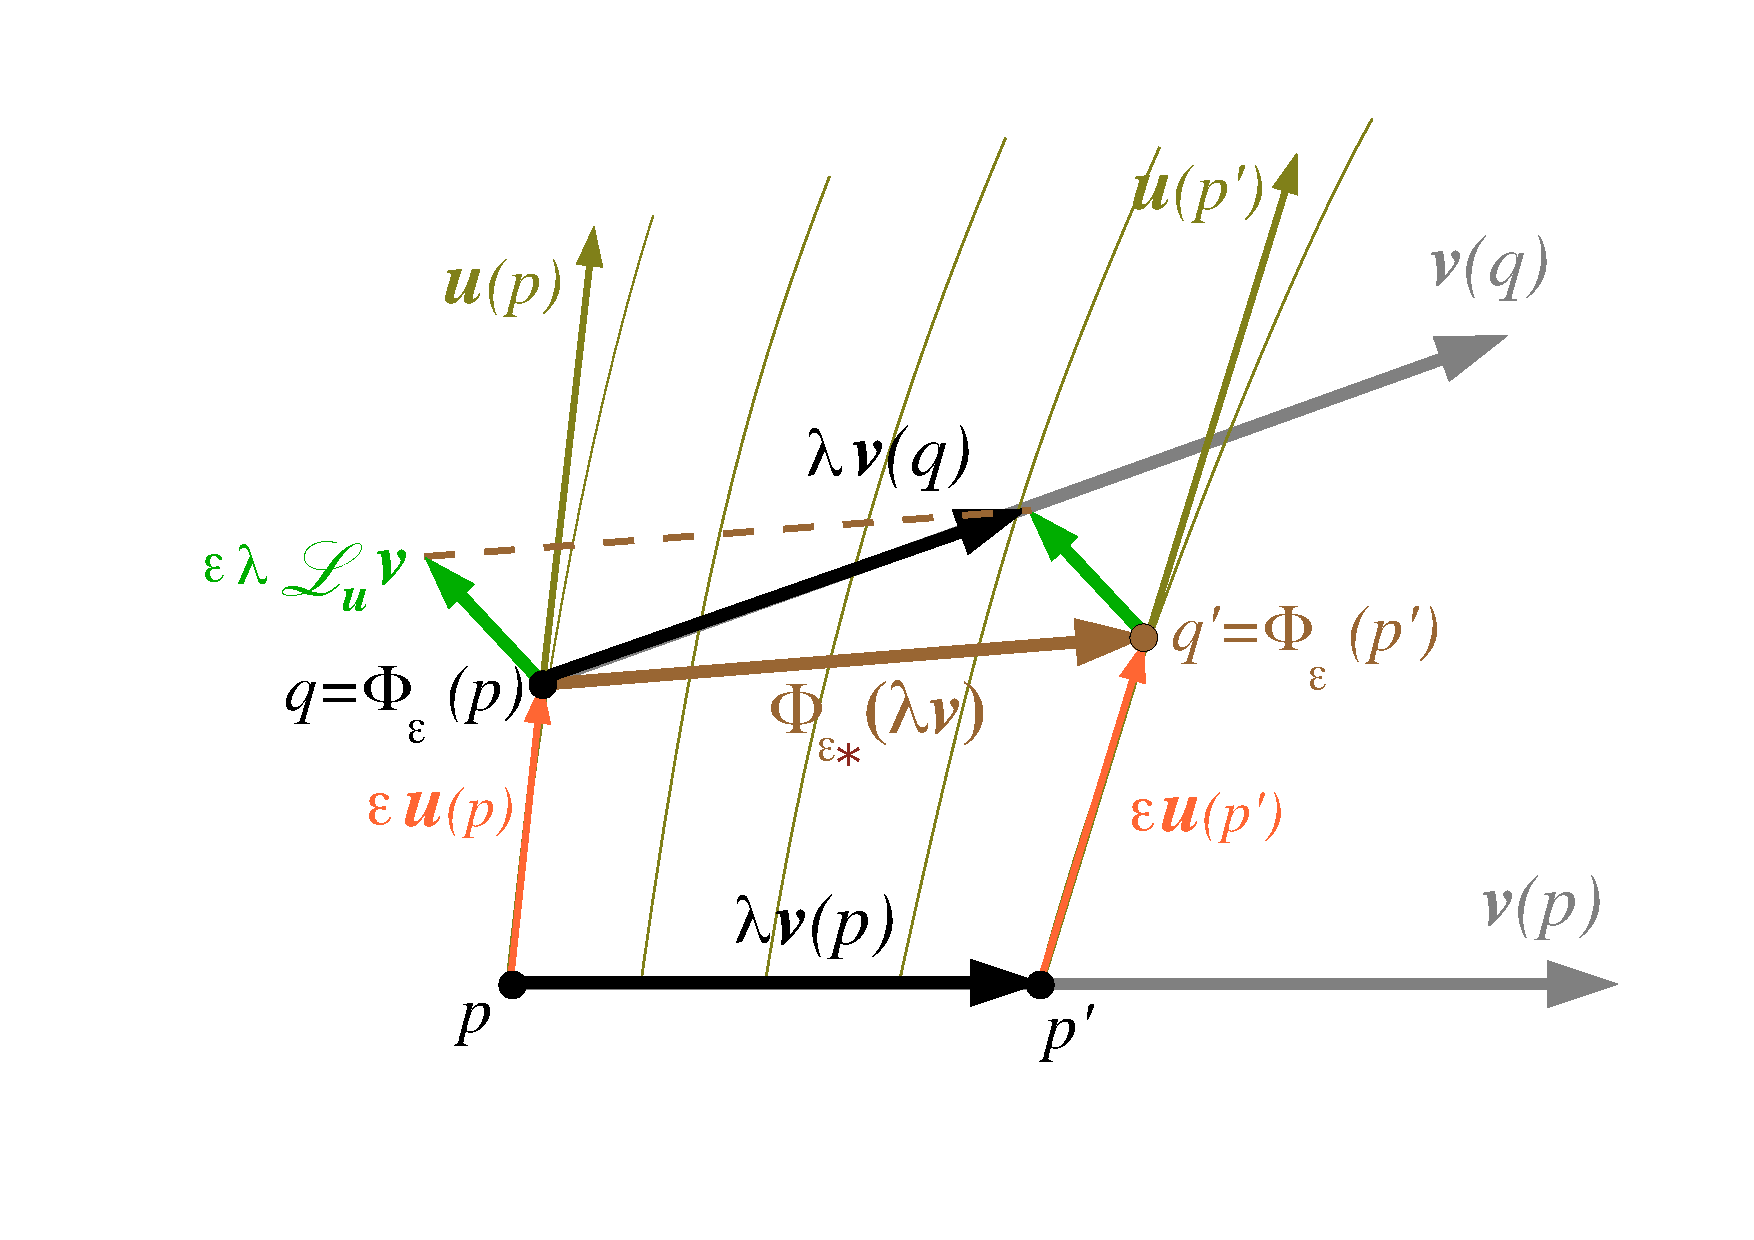
\includegraphics[width=0.6\textwidth]{bas_lie_deriv.pdf}}
\caption[]{\label{f:bas:deriv}
\footnotesize
Geometrical construction of the Lie derivative of a
vector field $\w{v}$ along a vector field $\w{u}$:
given a small parameter $\lambda$, each extremity of the arrow
$\lambda\w{v}$ is dragged by some small parameter $\varepsilon$
along $\w{u}$, to form
the vector denoted by $\Phi_{\veps*}(\lambda\w{v})$. The latter is then compared with
the actual value of $\lambda\w{v}$ at the point $q$, the difference (divided
by $\lambda\varepsilon$) defining the Lie derivative $\Lie{u}\w{v}$.}
\end{figure}


Let us consider a coordinate system $(x^\alpha)$ adapted to the
field $\w{u}$ in the sense that $\w{u}=\wpar_0$, where $\wpar_0$ is the first
vector of the natural basis associated with the coordinates $(x^\alpha)$.
We have, from the definitions of points $q$, $p'$ and $q'$,
\bea
  & & x^\alpha(q) = x^\alpha(p)+\varepsilon \delta^\alpha_{\ \ 0}  \nonumber \\
  & & x^\alpha(p')= x^\alpha(p)+ \lambda v^\alpha(p) \nonumber \\
  & & x^\alpha(q')= x^\alpha(p')+\varepsilon \delta^\alpha_{\ \ 0} ,\nonumber
\eea
so that
\[
  (qq')^\alpha = x^\alpha(p')-x^\alpha(p) = \lambda v^\alpha(p) .
\]
Accordingly, (\ref{e:bas:def_Phi_eps}) and (\ref{e:bas:def_Lie_der}) result in
\bea
  \left( \Lie{u} \w{v} \right)^\alpha & = &\lim_{\varepsilon\rightarrow 0} \frac{1}{\varepsilon}
  \left[ v^\alpha(q) - v^\alpha(p) \right] \nonumber \\
  & = &
  \lim_{\varepsilon\rightarrow 0} \frac{1}{\varepsilon}
  \left[ v^\alpha(x^0+\varepsilon,\; x^1,\; \ldots,\; x^{n-1}) -
  v^\alpha(x^0, \; x^1,\; \ldots,\; x^{n-1}) \right] . \nonumber
\eea
Hence, in adapted coordinates, the Lie derivative is simply obtained by taking the partial derivative of the vector components
with respect to $x^0$:
\be \label{e:bas:Lie_adapted_vec}
    \Liec{u} v^\alpha  = \der{v^\alpha}{x^0} ,
\ee
where we have used the standard notation for the components of a Lie derivative:
$\Liec{u} v^\alpha := \left( \Lie{u} \w{v} \right)^\alpha$.
Besides, using the fact that the components of $\w{u}$
are $u^\alpha=(1,0,\ldots,0)$ in the adapted coordinate system, we notice that the components
of the commutator of $\w{u}$ and $\w{v}$, as given by (\ref{e:bas:commut_comp}), are
\[
  [\w{u},\w{v}]^\alpha = \der{v^\alpha}{x^0} .
\]
This is exactly (\ref{e:bas:Lie_adapted_vec}): $[\w{u},\w{v}]^\alpha = \Liec{u} v^\alpha$. We conclude that the Lie derivative of a vector with respect to another
one is actually nothing but the commutator of these two vectors:
\be \label{e:bas:Lie_commut}
    \encadre{ \Lie{u} \w{v} = [\w{u},\w{v}] } .
\ee
Thanks to formula (\ref{e:bas:commut_comp}), we may then express the components of the Lie
derivative in an arbitrary coordinate system:
\be \label{e:bas:Lie_vect}
    \encadre{ \Liec{u} v^\alpha = u^\mu \der{v^\alpha}{x^\mu}
    - v^\mu \der{u^\alpha}{x^\mu} } .
\ee

Thanks to the symmetry property of the Christoffel symbols,
the partial derivatives in Eq.~(\ref{e:bas:Lie_vect}) can be
replaced by the Levi-Civita connection
$\wnab$ associated with some metric $\w{g}$, yielding
\be \label{e:bas:Lie_vect_nab}
  \Liec{u} v^\alpha = u^\mu \nabla_\mu v^\alpha
    - v^\mu \nabla_\mu u^\alpha .
\ee

\subsubsection{Generalization to any tensor field} \label{s:bas:lie_der_tensor}

If $\w{T}$ is tensor field of type $(0,\ell)$ on $\M$ (with $\ell \geq 1$)
its \defin{pullback}\index{pullback}
by the flow map
$\Phi_\varepsilon$ is the tensor field $\Phi_\veps^*\w{T}$ of type $(0,\ell)$
defined by applying $\w{T}$ to pushforwarded vectors:
\be \label{e:bas:def_pullback}
    \forall (\w{v}_1,\ldots,\w{v}_\ell)\in (T_p\M)^\ell,\quad
    \left. \Phi_\veps^*\w{T}\right| _p(\w{v}_1,\ldots,\w{v}_\ell) :=
        \left.\w{T}\right| _{\Phi_\varepsilon(p)} \left( \Phi_{\veps*}(\w{v}_1),
         \ldots, \Phi_{\veps*}(\w{v}_\ell) \right) .
\ee
The \defin{Lie derivative} of $\w{T}$ along $\w{u}$ is then defined
by comparing the pullback image at some point $p$ to the actual value
of $\w{\omega}$ at the same point:
\be \label{e:bas:def_Lie_der_covar}
    \encadre{ \Lie{u} \w{T} := \lim_{\varepsilon\rightarrow 0} \frac{1}{\varepsilon}
    \left( \Phi_\varepsilon^*\w{T} - \w{T} \right) }.
\ee

Finally, the Lie derivative is extended to any tensor field by (i) demanding that for
a scalar field $f$, $\Lie{u} f = \langle\wnab f,\w{u}\rangle$ and (ii) using the Leibniz
rule. As a result, the Lie derivative $\Lie{u}\w{T}$ of a tensor field $\w{T}$ of type
$(k,\ell)$ is a tensor field of the same type, the components of which
with respect to a given coordinate system $(x^\alpha)$ are
\bea
\Liec{u} T^{\alpha_1\ldots\alpha_k}_{\qquad\ \; \beta_1\ldots\beta_\ell} &=&
u^\mu \der{}{x^\mu} T^{\alpha_1\ldots\alpha_k}_{\qquad\ \; \beta_1\ldots\beta_\ell}
- \sum_{i=1}^k T^{\alpha_1\ldots
\!{{{\scriptstyle i\atop\downarrow}\atop \scriptstyle\sigma}\atop\ }\!\!
\ldots\alpha_k}_{\qquad\ \ \ \  \  \  \; \beta_1\ldots\beta_\ell}
 \; \der{u^{\alpha_i}}{x^\sigma} \nonumber \\
 & &  +  \sum_{i=1}^\ell T^{\alpha_1\ldots\alpha_k}_{\qquad\ \; \beta_1\ldots
\!{\ \atop {\scriptstyle\sigma \atop {\uparrow\atop \scriptstyle i}} }\!\!
\ldots\beta_\ell}
\; \der{u^{\sigma}}{x^{\beta_i}} . \label{e:Lie_der_comp}
\eea
In particular, for a 1-form,
\be \label{e:Lie_der_1form}
    \Liec{u} \omega_\alpha = u^\mu \der{\omega_\alpha}{x^\mu}
    + \omega_\mu \der{u^\mu}{x^\alpha} .
\ee
As for the vector case [Eq.~(\ref{e:bas:Lie_vect})], the
partial derivatives in Eq.~(\ref{e:Lie_der_comp}) can be
replaced by the covariant derivative $\wnab$ (or any other connection without torsion),
yielding
\bea
\Liec{u} T^{\alpha_1\ldots\alpha_k}_{\qquad\ \; \beta_1\ldots\beta_\ell} &=&
u^\mu \nabla_\mu T^{\alpha_1\ldots\alpha_k}_{\qquad\ \; \beta_1\ldots\beta_\ell}
- \sum_{i=1}^k T^{\alpha_1\ldots
\!{{{\scriptstyle i\atop\downarrow}\atop \scriptstyle\sigma}\atop\ }\!\!
\ldots\alpha_k}_{\qquad\ \ \ \  \  \  \; \beta_1\ldots\beta_\ell}
 \; \nabla_\sigma u^{\alpha_i} \nonumber \\
 & & +  \sum_{i=1}^\ell T^{\alpha_1\ldots\alpha_k}_{\qquad\ \; \beta_1\ldots
\!{\ \atop {\scriptstyle\sigma \atop {\uparrow\atop \scriptstyle i}} }\!\!
\ldots\beta_\ell}
\; \nabla_{\beta_i} u^{\sigma} . \label{e:bas:Lie_der_comp_nab}
\eea
A special case of the above formula is worth considering, namely that of the
metric tensor $\w{g}$:
\[
    \Liec{u} g_{\alpha\beta} = u^\mu \underbrace{\nabla_\mu g_{\alpha\beta}}_{0}
        + \underbrace{g_{\sigma\beta} \nabla_\alpha u^\sigma}_{\nabla_\alpha u_\beta}
        + \underbrace{g_{\alpha\sigma} \nabla_\beta u^\sigma}_{\nabla_\beta u_\alpha} .
\]
Hence, one gets the so-called \defin{Killing expression}\index{Killing!expression}
of the Lie derivative of the metric tensor:
\be \label{e:bas:Lie_g_Killing}
   \encadre{ \Liec{u} g_{\alpha\beta} = \nabla_\alpha u_\beta + \nabla_\beta u_\alpha }.
\ee

In adapted coordinates, we have, similarly to Eq.~(\ref{e:bas:Lie_adapted_vec}),
\be \label{e:bas:Lie_adapted}
    \Liec{u} T^{\alpha_1\ldots\alpha_k}_{\qquad\ \; \beta_1\ldots\beta_\ell}
     = \der{}{x^0} T^{\alpha_1\ldots\alpha_k}_{\qquad\ \; \beta_1\ldots\beta_\ell}
     \qquad \mbox{(coordinates adapted to $\w{u}$)}.
\ee
Note that this formula is a direct consequence of (\ref{e:Lie_der_comp})
since in adapted coordinates, $u^\alpha = (1,0,\ldots,0)$, so that
$u^\mu \dert{}{x^\mu} = \dert{}{x^0}$ and $\dert{u^\alpha}{x^\beta} = 0$.


\subsection{Exterior derivative} \label{s:bas:ext_deriv}

In Sec.~\ref{s:bas:fields}, we have introduced the
\emph{differential forms}\index{differential!form}\index{form!differential}
or \emph{$p$-forms}
as tensor fields of type $(0,p)$, with $p\ge 0$,
that are antisymmetric in all their arguments as soon as $p\ge 2$.
Differential forms play a special role in the theory of integration on
manifolds. Indeed, the primary definition of an integral over a manifold of
dimension $n$ is the integral of a $n$-form. The Levi-Civita tensor
$\w{\epsilon}$
introduced in Sec.~\ref{s:bas:Levi-Civita_tensor} is a $n$-form, whose integral
gives the volume with respect to the metric $\w{g}$.
Regarding physics, the
electromagnetic field is a 2-form $\w{F}$ (cf. Sec.~\ref{e:fra:electrovacuum});
in relativistic hydrodynamics, the vorticity of a fluid is also described by a 2-form
(see e.g. \cite{Gourg13}).

Being tensor fields, differential forms are subject to the covariant
and Lie derivatives discussed above. But, in addition, they are subject to a third kind
of derivative, called the \emph{exterior derivative}.
The \defin{exterior derivative}\index{exterior!derivative}\index{derivative!exterior}
 of a $p$-form $\w{\omega}$ is a
$(p+1)$-form which is denoted $\dd\w{\omega}$ and whose components
with respect to a given coordinate system $(x^\alpha)$ are defined by
\bea
    \mbox{0-form (scalar field)} & : & (\dd\w{\omega})_\alpha :=
        \der{\omega}{x^\alpha} \label{e:bas:def_ext_0f} \\
    \mbox{1-form} & : & (\dd\w{\omega})_{\alpha\beta} :=
    \der{\omega_\beta}{x^\alpha} - \der{\omega_\alpha}{x^\beta}
             \label{e:bas:def_ext_1f} \\
    \mbox{2-form} & : & (\dd\w{\omega})_{\alpha\beta\gamma} :=
    \der{\omega_{\beta\gamma}}{x^\alpha} +
    \der{\omega_{\gamma\alpha}}{x^\beta} +
    \der{\omega_{\alpha\beta}}{x^\gamma} \label{e:bas:def_ext_2f} \\
    \mbox{etc...} \nonumber
\eea
It can be easily checked that these formul\ae, although expressed in terms of
partial derivatives of components in a coordinate system, do define tensor fields.
Moreover, the result is clearly antisymmetric (assuming that $\w{\omega}$ is), so
that we end up with $(p+1)$-forms.
Notice that for a scalar field (0-form), the exterior derivative is nothing but the
differential 1-form $\dd f$ already defined in Sec.~\ref{s:bas:linear_form}.
Notice also that the exterior derivative appeals only to the
manifold structure. It does not depend upon the metric tensor  $\w{g}$, nor upon
any other extra structure on $\M$.

\begin{remark}
Although the exterior derivative does not depend on the metric $\w{g}$ and
hence on the Levi-Civita connection $\wnab$, one may replace
all partial derivatives in the formul\ae\
(\ref{e:bas:def_ext_0f})-(\ref{e:bas:def_ext_2f}) by covariant derivatives:
\bea
    \mbox{0-form} & : & (\dd\w{\omega})_\alpha =
        \nabla_\alpha \omega \label{e:bas:def_ext_0f_nab} \\
    \mbox{1-form} & : & (\dd\w{\omega})_{\alpha\beta} =
        \nabla_\alpha \omega_\beta - \nabla_\beta \omega_\alpha
            \label{e:bas:def_ext_1f_nab} \\
    \mbox{2-form} & : & (\dd\w{\omega})_{\alpha\beta\gamma} =
    \nabla_\alpha\omega_{\beta\gamma} +
    \nabla_\beta\omega_{\gamma\alpha} +
    \nabla_\gamma\omega_{\alpha\beta} \label{e:bas:def_ext_2f_nab}
\eea
The above identities hold thanks to the symmetry of the Christoffel symbols
on their last two indices (and thanks to (\ref{e:bas:grad_f_der_f}) for
a 0-form).
\end{remark}

A fundamental property of the exterior derivative is to be nilpotent:
\be \label{e:ext_der_nilpot}
    \encadre{ \dd\dd\w{\omega} = 0 }.
\ee
A $p$-form $\w{\omega}$ is said to be \defin{closed}\index{closed!differential form} iff $\dd\w{\omega}=0$,
and \defin{exact}\index{exact diff. form} iff there exists a $(p-1)$-form $\w{\sigma}$ such that
$\w{\omega} = \dd\w{\sigma}$. From property (\ref{e:ext_der_nilpot}),
any exact $p$-form is closed. The Poincaré lemma states that the converse is true,
at least locally.

The exterior derivative enters in the well known \defin{Stokes' theorem}\index{Stokes!theorem}: if $\mathcal{D}$
is a submanifold of $\M$ of dimension $d$ that has a boundary (denoted $\partial\mathcal{D}$), then for any $(d-1)$-form $\w{\omega}$,
\be \label{e:bas:Stokes}
    \int_{\partial\mathcal{D}} \w{\omega} =
    \int_{\mathcal{D}} \dd\w{\omega} .
\ee
Note that $\partial\mathcal{D}$ is a manifold of dimension $d-1$ and
$\dd\w{\omega}$ is a $d$-form, so that each side of
(\ref{e:bas:Stokes}) is (of course !) a well-defined quantity,
as the integral of a $p$-form over a $p$-dimensional manifold.

Another very important formula involving the exterior derivative is
the \defin{Cartan identity}\index{Cartan!identity}, which states that the
Lie derivative of a differential form
$\w{\omega}$ along a vector field $\w{u}$ is expressible as
\be \label{e:bas:Cartan}
    \encadre{ \Lie{u}\w{\omega} = \w{u}\cdot\dd\w{\omega}
    + \dd(\w{u}\cdot\w{\omega}) }.
\ee
In the above formula, a dot denotes the contraction on adjacent indices, i.e.
$\w{u}\cdot\w{\omega}$ is the $(p-1)$-form $\w{\omega}(\w{u},.,\ldots,.)$,
with the $p-1$ last slots remaining free. Notice that if $\w{\omega}$ is
a 1-form, Eq.~(\ref{e:bas:Cartan}) is readily obtained
by combining Eqs.~(\ref{e:Lie_der_1form}),
(\ref{e:bas:def_ext_0f}) and (\ref{e:bas:def_ext_1f}).
An immediate consequence of the Cartan identity and the nilpotence property
(\ref{e:ext_der_nilpot}) is that the Lie derivative
and the exterior derivative commute, i.e. for any vector field $\w{u}$
and any $p$-form $\w{\omega}$:
\be \label{e:bas:Lie_ext_commute}
    \Lie{u} \dd \w{\omega} = \dd \, \Lie{u}\! \w{\omega} .
\ee

%%%%%%%%%%%%%%%%%%%%%%%%%%%%%%%%%%%%%%%%%%%%%%%%%%%%%%%%%%%%%%%%%%%%%%%%%%%%%%%

\section{Curvature} \label{s:bas:curvat}

\subsection{General definition}

The \defin{Riemann curvature tensor}\index{Riemann!curvature}\index{curvature!tensor} of
an affine connection $\w{\nabla}$ is defined by
\be \label{e:bas:def_Riemann}
     \begin{array}{cccc}
    \mathrm{\bf Riem} \ : & \mathfrak{X}^*(\M)\times\mathfrak{X}(\M)^3 &
    \longrightarrow & C^\infty(\M,\R) \\
        & (\w{\omega},\w{w},\w{u},\w{v})
        & \longmapsto & \bigg\langle \w{\omega} , \
                \w{\nabla}_{\w{u}} \w{\nabla}_{\w{v}} \w{w}
        -  \w{\nabla}_{\w{v}} \w{\nabla}_{\w{u}} \w{w}
        - \w{\nabla}_{[\w{u},\w{v}]} \w{w} \bigg\rangle ,
    \end{array}
\ee
where $\mathfrak{X}^*(\M)$ stands for the space of 1-forms on $\M$, $\mathfrak{X}(\M)$ for the space of vector
fields on $\M$ and  $C^\infty(\M,\R)$ for the space of
smooth scalar fields on $\M$. The above
formula does define a tensor field on $\M$, i.e. the value
of $\mathrm{\bf Riem}(\w{\omega},\w{w},\w{u},\w{v})$ at a given
point $p\in\M$ depends only upon the values of the fields
$\w{\omega}$, $\w{w}$, $\w{u}$ and $\w{v}$ at $p$ and not
upon their behaviours away from $p$, as the covariant derivatives in
Eq.~(\ref{e:bas:def_Riemann}) might suggest.
We denote the components of this tensor in
a given basis $(\w{e}_\alpha)$, not by
${\rm Riem}^\gamma_{\ \  \delta \alpha\beta}$, but by
$R^\gamma_{\ \  \delta \alpha\beta}$.
The definition (\ref{e:bas:def_Riemann}) leads then to the
following expression, named the \defin{Ricci identity}\index{Ricci!identity}:
\be \label{e:bas:Ricci_ident}
    \forall\w{w}\in\mathfrak{X}(\M),\quad
        \left(\nabla_\alpha\nabla_\beta
        - \nabla_\beta\nabla_\alpha\right) w^\gamma
        = R^\gamma_{\ \  \mu \alpha\beta} \, w^\mu .
\ee
\begin{remark}
In view of this identity, one may say that the Riemann tensor measures the lack of
commutativity of two successive covariant derivatives of a vector field.
On the opposite,
for a scalar field and a torsion-free connection,
two successive covariant derivatives always commute [cf. Eq.~(\ref{e:bas:torsion-free})].
\end{remark}
In a coordinate basis, the components of the Riemann tensor are given in terms of the connection
coefficients by
\be \label{e:bas:Riemann_comp}
    \encadre{ R^\alpha_{\ \  \beta\mu\nu}  =
    \der{\Gamma^\alpha_{\ \  \beta\nu}}{x^\mu}
    - \der{\Gamma^\alpha_{\ \  \beta\mu}}{x^\nu}
    + \Gamma^\alpha_{\ \  \sigma\mu} \Gamma^\sigma_{\ \  \beta\nu}
    - \Gamma^\alpha_{\ \  \sigma\nu} \Gamma^\sigma_{\ \  \beta\mu}  } .
\ee

From the definition (\ref{e:bas:def_Riemann}), the Riemann tensor is
clearly antisymmetric with respect to its last two arguments $(\w{u},\w{v})$:
\be \label{e:bas:Riemann_antisym34}
  \mathrm{\bf Riem}(.,.,\w{u},\w{v}) = - \mathrm{\bf Riem}(.,.,\w{v},\w{u}) .
\ee
In addition, it satisfies the cyclic property
\be \label{e:bas:Riemann_cyclic}
\mathrm{\bf Riem}(.,\w{u},\w{v},\w{w})
+\mathrm{\bf Riem}(.,\w{w},\w{u},\w{v})
+\mathrm{\bf Riem}(.,\w{v},\w{w},\w{u}) = 0 .
\ee
The covariant derivatives of the Riemann tensor obeys the \defin{Bianchi identity}\index{Bianchi identity}
\be \label{e:bas:Bianchi}
    \encadre{ \nabla_\rho  R^\alpha_{\ \  \beta\mu\nu}
    + \nabla_\mu R^\alpha_{\ \ \beta\nu\rho}
    + \nabla_\nu R^\alpha_{\ \ \beta\rho\mu} =0 }.
\ee

\subsection{Case of a pseudo-Riemannian manifold}

The Riemann tensor of the Levi-Civita connection obeys the additional antisymmetry:
\be \label{e:bas:Riemann_antisym12}
    \mathrm{\bf Riem}(\w{\omega},\w{w},.,.)
    = - \mathrm{\bf Riem}(\uu{w},\vw{\omega},.,.) .
\ee
Combined with (\ref{e:bas:Riemann_antisym34}) and (\ref{e:bas:Riemann_cyclic}), this implies
the symmetry property
\be \label{e:bas:Riemann_sym}
  \mathrm{\bf Riem}(\w{\omega},\w{w},\w{u},\w{v}) =
  \mathrm{\bf Riem}(\uu{u},\w{v},\vw{\omega},\w{w}) .
\ee

A pseudo-Riemannian manifold $(\M,\w{g})$ with a vanishing Riemann tensor is called
a \defin{flat manifold}\index{flat!manifold}; in this case, $\w{g}$ is said to be
a \defin{flat metric}\index{flat!metric}. If in addition, it has a Riemannian signature,
$\w{g}$ is called an
\defin{Euclidean metric}\index{Euclidean!metric}.

\subsection{Ricci tensor} \label{s:bas:Ricci_tensor}

The \defin{Ricci tensor}\index{Ricci!tensor} of the affine connection $\wnab$ is
the field of bilinear forms $\w{R}$ defined by
\be \label{e:bas:def_Ricci}
     \begin{array}{cccc}
    \w{R} \ : & \mathfrak{X}(\M)\times\mathfrak{X}(\M) &
    \longrightarrow & C^\infty(\M,\R) \\
        & (\w{u},\w{v})
        & \longmapsto &
                \mathrm{\bf Riem}(\w{e}^\mu,\w{u},\w{e}_\mu,\w{v}) ,
    \end{array}
\ee
where $(\w{e}_\alpha)$ is a vector frame on $\M$ and $(\w{e}^\alpha)$
its dual counterpart.
This definition is independent of the choice of $(\w{e}_\alpha)$.
In terms of components:
\be \label{e:bas:def_Ricci_comp}
    \encadre{ R_{\alpha\beta} := R^\mu_{\ \  \alpha\mu\beta} }.
\ee
\begin{remark}
Following the standard usage, we denote the components
of the Riemann and Ricci tensors by the same letter $R$, the
number of indices allowing us to distinguish between the two tensors.
On the other hand, we are using different symbols, $\mathrm{\bf Riem}$ and
$\w{R}$, when employing the index-free notation.
\end{remark}

For the Levi-Civita connection associated with the metric $\w{g}$, the property (\ref{e:bas:Riemann_sym}) implies that the Ricci tensor is symmetric:
\be
  \w{R}(\w{u},\w{v}) = \w{R}(\w{v},\w{u}) .
\ee
In addition, one defines the
\defin{Ricci scalar}\index{Ricci!scalar}
(also called \defin{scalar curvature}\index{scalar!curvature}\index{curvature!scalar})
as the trace of the Ricci tensor with respect to the metric $\w{g}$:
\be \label{e:bas:def_Ricci_scal}
  R :=g^{\mu\nu} R_{\mu\nu} .
\ee
The Bianchi identity (\ref{e:bas:Bianchi}) implies the divergence-free property
\be \label{e:bas:Bianchi_contr}
  \encadre{ \wnab\cdot\vw{G} = 0 },
\ee
where $\vw{G}$ in the type-$(1,1)$ tensor associated by metric duality
[cf. (\ref{e:bas:arrow_endo})] to
the \defin{Einstein tensor}\index{Einstein!tensor}:
\be \label{e:bas:Einstein_tensor}
  \encadre{ \w{G} := \w{R} - \frac{1}{2} R\, \w{g} } .
\ee
Equation~(\ref{e:bas:Bianchi_contr}) is called the \defin{contracted Bianchi identity}\index{contracted!Bianchi identity}\index{Bianchi identity!contracted}.

\subsection{Weyl tensor} \label{s:bas:Weyl}

Let $(\M,\w{g})$ be a pseudo-Riemannian manifold of dimension $n$.

For $n=1$, the Riemann tensor vanishes identically, i.e. $(\M,\w{g})$  is
necessarily flat.
The reader having in mind a curved line in the Euclidean plane $\R^2$ might be
surprised by the above statement. This is because the Riemann tensor
represents the  \emph{intrinsic} curvature\index{intrinsic curvature}\index{curvature!intrinsic} of a manifold. For a curved line $\Li$, the
curvature that is not vanishing is the
\emph{extrinsic} curvature\index{extrinsic curvature}\index{curvature!extrinsic --}, i.e. the
curvature resulting from the embedding of $\Li$ in $\R^2$.

For $n=2$, the Riemann tensor is entirely determined by the
Ricci scalar $R$, according to the formula:
\be \label{e:bas:Riem_n_2}
  R^\gamma_{\ \; \delta\alpha\beta} =  \frac{R}{2} \left(
    \delta^\gamma_{\ \  \alpha} \, g_{\delta\beta}   -
    \delta^\gamma_{\ \  \beta} \, g_{\delta\alpha}
         \right) \qquad (n=2) .
\ee

For $n=3$, the Riemann tensor is entirely determined by the
Ricci tensor, according to
\bea
    R^\gamma_{\ \; \delta\alpha\beta}   & =&
     R^\gamma_{\ \  \alpha} \, g_{\delta\beta}
       - R^\gamma_{\ \  \beta}\,  g_{\delta\alpha}
       + \delta^\gamma_{\ \  \alpha} \, R_{\delta\beta}
       - \delta^\gamma_{\ \  \beta}  \, R_{\delta\alpha}
  \nonumber \\
     & &  + \frac{R}{2} \left(
  \delta^\gamma_{\ \  \beta} \, g_{\delta\alpha}
       - \delta^\gamma_{\ \  \alpha} \, g_{\delta\beta}   \right)
   \qquad (n=3) . \label{e:bas:Riem_dim_3}
\eea

For $n\geq 4$, the Riemann tensor can
be split into (i) a ``trace-trace'' part, represented
by the Ricci scalar $R$ [Eq.~(\ref{e:bas:def_Ricci_scal})],
(ii) a ``trace'' part,
represented by the Ricci tensor $\w{R}$
[Eq.~(\ref{e:bas:def_Ricci_comp})], and (iii) a ``traceless'' part,
which is constituted by the \defin{Weyl conformal curvature tensor}\index{Weyl curvature tensor}\index{conformal!curvature}, $\w{C}$:
\bea
    R^\gamma_{\ \; \delta\alpha\beta}   & = &
        C^\gamma_{\ \; \delta\alpha\beta}
    + \frac{1}{n-2} \left( R^\gamma_{\ \  \alpha} \, g_{\delta\beta}
       - R^\gamma_{\ \  \beta}\,  g_{\delta\alpha}
       + \delta^\gamma_{\ \  \alpha} \, R_{\delta\beta}
       - \delta^\gamma_{\ \  \beta} \, R_{\delta\alpha}   \right)
                            \nonumber \\
     &&   + \frac{1}{(n-1)(n-2)} R \left(
  \delta^\gamma_{\ \  \beta} \, g_{\delta\alpha}
       - \delta^\gamma_{\ \  \alpha} \, g_{\delta\beta}   \right) . \label{e:bas:Weyl}
\eea
The above relation may be taken as the definition of $\w{C}$.
It implies that $\w{C}$ is traceless: $C^\mu_{\ \  \alpha\mu\beta}=0$.
The other possible traces are zero thanks to the symmetry properties of
the Riemann tensor.
\begin{remark}
The decomposition (\ref{e:bas:Weyl}) is meaningful for $n=3$ as well, but then
it implies that the Weyl tensor vanishes identically [compare with (\ref{e:bas:Riem_dim_3})].
\end{remark}

